%%
%% This is file `thesis.tex',
%% generated with the docstrip utility.
%%
%% The original source files were:
%%
%% nudtpaper.dtx  (with options: `thesis')
%% 
%% This is a generated file.
%% 
%% Copyright (C) 2020 by Liu Benyuan <liubenyuan@gmail.com>
%% 
%% This file may be distributed and/or modified under the
%% conditions of the LaTeX Project Public License, either version 1.3a
%% of this license or (at your option) any later version.
%% The latest version of this license is in:
%% 
%% http://www.latex-project.org/lppl.txt
%% 
%% and version 1.3a or later is part of all distributions of LaTeX
%% version 2004/10/01 or later.
%% 
%% To produce the documentation run the original source files ending with `.dtx'
%% through LaTeX.
%% 
%% Any Suggestions : LiuBenYuan <liubenyuan@gmail.com>
%% Thanks Xue Ruini <xueruini@gmail.com> for the thuthesis class!
%% Thanks sofoot for the original NUDT paper class!
%% 
%1. 规范硕士导言
 \documentclass[master,ttf]{nudtpaper}
%2. 规范博士导言
% \documentclass[doctor,twoside,ttf]{nudtpaper}
%3. 建议使用OTF字体获得较好的页面显示效果
%   OTF字体从网上获得,各个系统名称统一。
%   如果你下载的是最新的(1201)OTF英文字体,建议修改nudtpaper.cls,使用
%   Times New Roman PS Std
% \documentclass[doctor,twoside,otf]{nudtpaper}
%   另外,新版的论文模板提供了方正字体选项FZ,效果也不错哦
% \documentclass[doctor,twoside,fz]{nudtpaper}
%4. 如果想生成盲评,传递anon即可,仍需修改个人成果部分
% \documentclass[master,otf,anon]{nudtpaper}
%
%5. 参考文献若用biblatex生成,则使用biber选项
% \documentclass[master,biber]{nudtpaper}
%
%6. 简历中的论文和成果用biblatex参考文献方式生成,则使用resumebib选项
% \documentclass[master,biber,resumebib]{nudtpaper}
%
%\documentclass[doctor,twoside,biber,resumebib,fz]{nudtpaper}
\usepackage{mynudt}

\classification{TP957}
\serialno{0123456}
\confidentiality{公开}
\UDC{}
\title{国防科大学位论文\LaTeX{}模板\\
使用手册}
\displaytitle{国防科技大学学位论文\LaTeX{}模板}
\author{张三}
\zhdate{\zhtoday}
\entitle{How to Use the \LaTeX{} Document Class for NUDT Dissertations}
\enauthor{ZHANG San}
\endate{\entoday}
\subject{通信与信息工程}
\ensubject{Information and Communication Engineering}
\researchfield{自动目标识别与模糊工程}
\supervisor{李四\quad{}教授}
\cosupervisor{王五\quad{}副教授} % 没有就空着
\ensupervisor{Prof. LI Si}
\encosupervisor{} % 没有就空着
\papertype{工学}
\enpapertype{Engineering}
% 加入makenomenclature命令可用nomencl制作符号列表。

\begin{document}
\graphicspath{{figures/}}
% 制作封面,生成目录,插入摘要,插入符号列表 \\
% 默认符号列表使用denotation.tex,如果要使用nomencl \\
% 需要注释掉denotation,并取消下面两个命令的注释。 \\
% cleardoublepage% \\
% printnomenclature% \\
\maketitle
\frontmatter
\tableofcontents
\listoftables
\listoffigures

%如果不是送审论文,则将true改为false即可
\newif\ifreview\reviewfalse

\midmatter
\begin{cabstract}

气动优化设计是航空航天飞行器设计等应用的重要组成部分,随着飞行器产业的发展和应对复杂现实环境需求的提升,
气动优化往往涉及许多相互交织影响的因素,容易导致设计优化空间“爆炸”。全阶的计算流体力学(CFD)方法能够针对特定流动状态进行高精度的模拟,但往往耗时较长难以进行全面的设计空间探索;虽然基于传统机器学习方法的优化技术在构建代理模型、降阶模型等方面有广泛的应用,
但这类方法多适用于简单气动优化问题,具有一定的局限性。
近年来,深度学习相关研究不断深入并推动诸多应用领域进一步发展,为提升气动优化效率,
构建高效、准确的气动评估方法提供了新的途径。本文主要研究内容如下:

\begin{itemize}
	\item[(1)] 通过对比研究气动流场模拟任务和图像回归预测任务的相似性和不同点,本文提出了一种基于深度卷积网络的气动流场预测方法。首先,针对流场数据的表示问题,提出基于笛卡尔网络的流场数据表示方法,将流场数据转化为深度神经网络可以接受的形式。
	其次,针对边界层等区域流场物理量变化大、包含重要信息多特点,本文提出了嵌入注意力模块的深度卷积网络,能够有效学习该区域流动规律,提升模型预测准确率;基于流体运动遵循的质量守恒定律和动量守恒定律,设计了物理约束的损失函数,有效保证了深度学习预测模型预测结果和CFD求解器的物理一致性。为了全面的评估气动流场预测模型的性能,本文定义了新的性能指标,在测试集上的对比试验结果表明该方法能有效提升气动流场模拟效率,同时将预测误差控制在5\%以内。
	\item[(2)] 针对深度卷积网络难以处理非欧式空间流场数据的问题,本文提出了一种基于图神经网络的气动流场模拟加速方法。
	基于图结构对流场数据进行表示,能够有效减少数据转换过程中的信息丢失,实现流场几何外形、边界条件和流动控制变量的有效融合;
	基于图卷积网络的流模拟加速模块能够提取流场数据特征,为CFD求解器提供接近收敛状态的初始场,减少CFD迭代计算的时间。
	实验结果表明该方法能够在加速气动流场模拟的同时,从根本上保证了模拟结果的有效性。
	
\end{itemize}

本文针对飞行器气动优化设计中的典型问题,基于深度学习技术和方法,提出针对流场数据的表示方法,搭建气动流场预测模型和气动流场模拟加速模型,通过嵌入物理约束和融合传统CFD方法进一步优化模型预测结果,有效提升气动流场模拟效率,为基于深度学习的智能气动流场和气动性能预测技术在复杂飞行器气动优化设计中的应用奠定基础。

\end{cabstract}
\ckeywords{气动优化; 计算流体力学; 深度学习; 图神经网络; 物理一致性}



\begin{eabstract}
National University of Defense Technology is a comprehensive national key university based in Changsha, %
Hunan Province, China. It is under the dual supervision of the Ministry of National Defense %
and the Ministry of Education, designated for Project 211 and Project 985, %
the two national plans for facilitating the development of Chinese higher education. %

NUDT was originally founded in 1953 as the Military Academy of Engineering in Harbin of Heilongjiang Province. %
In 1970 the Academy of Engineering moved southwards to Changsha and was renamed Changsha Institute of Technology.%
 The Institute changed its name to National University of Defense Technology in 1978.

\end{eabstract}
\ekeywords{Aerodynamic Optimization; Computational Fluid Dynamics; Deep Learning; Graph  Neural  Network; Physical Consistency}


\input{data/denotation}

%书写正文,可以根据需要增添章节; 正文还包括致谢,参考文献与成果
\mainmatter
\chapter{绪论}
CFD数值模拟在航空航天飞行器气动优化设计等应用中发挥着重要作用,
但是全阶CFD模拟经济、时间成本高昂,限制了设计人员进行全面、快速的设计空间探索和设计迭代。为了以更省时省力、又快又好地获得最优解,机器学习等智能算法和技术在气动优化的寻优算法及构建代理模型、降阶模型等方面有广泛的应用,但是传统机器学习方法适用于处理低维数据,难以推广到复杂的CFD应用场景。随着人工智能领域的快速发展,以深度学习为代表的智能方法和技术在处理高维复杂数据上展现了强大的学习能力,从而为快速、精确气动评估提供了新思路和新方法。



\section{研究背景及意义}
计算流体力学( Computational Fluid Dynamics,CFD )
作为了解和探索流体运动的手段,在航空航天,交通运输,石油勘探,天气预测,水利工程和石油化工等工程领域发挥着极其重要的作用。近年来,随着计算机性能的提升,CFD的应用前景进一步扩大,渗透到生活的方方面面。小到吸管设计,大到汽车制造,生活中随处可见CFD的身影。在2020年新冠疫情期间,CFD研究者通过对喷嚏飞沫的流动状态进行研究,得出喷嚏飞沫可以漂浮8米远的结论,为疫情防控做出了重要的贡献\cite{JAMA-喷嚏}。

复杂飞行器气动优化设计是CFD的重要应用领域,以增升减阻为目标的气动优化是飞行器设计的重要组成部分。
如文献\cite{增升减阻ep}指出,对于某民航客机,起飞升阻比每提高1\%,可增加14个乘客;
着陆最大升力系数每增加1\%,则可增加22个乘客。
由此可见,提升气动优化效率,实现快速、精准的气动评估对于推动飞行器设计发展具有重要意义。
尽管传统的全阶CFD数值模拟可针对特定状态获得较高精度的评估结果,但是时间、经济等成本巨大。
为了以更省时省力、又快又好地获得最优解,许多研究者在优化设计时对原始模型进行简化处理,包括采用更为简单的代理模型\cite{代理模型}和降阶模型\cite{降阶模型},代替复杂的CFD评估过程,减少计算开销;引入基于机器学习的智能方法和技术等。因此,在保证模拟精度的基础上,不断地提升气动模拟的效率是数值模拟领域现阶段的研究热点,具有极大的实际应用价值。然而加速和优化气动评估目前面临着以下挑战:

\vspace{-0.2cm}
\begin{itemize}
	\item[(1)] 气动优化往往涉及许多相互交织影响的因素。以常见的超临界机翼优化为例,除需考虑巡航升阻力系数、升阻比、力矩系数等设
	计点性能外,抖振、阻力发散等非设计点动态特性也需考虑;同时,优化还存在一些必要约束,如机翼厚度、油箱容积、前后缘装置等。海量设计参数容易导致设计空间“爆炸”,仅依靠传统的CFD数值模拟极大地限制了对复杂飞行器进行全面的设计空间探索。
	\item[(2)] 机器学习等智能算法和技术,通过部分或者全部代替复杂的CFD评估过程,在原始模型简化处理方面有广泛的应用。
	然而,大部分机器学习技术借助于发展成熟的机器学习方法和技术,属于浅层学习方法,随着CFD所模拟的问题越加的复杂,其预测精度和应用范围相对有限。
	此外,传统机器学习算法复杂度将随着样本数量和模
	型精度的提高呈指数级增长,目前应用范围多限于一些容易获得训练样本的二维简单优化
	问题。

\end{itemize}

自2006年Hinton等提出深度信念网络\cite{深度信念网络}以来,在GPU、TPU等高性能计算机硬件的助力下,
以深度学习为代表的智能方法和技术迅速发展,成功应用于图像分类与识别,医疗诊断,视频预测,自然语言处理等诸多领域。
在学术界,深度学习算法和技术包括其相关应用也是世界各大研究实验室和顶尖大学的研究热点,
比如斯坦福大学、纽约大学、加拿大蒙特利尔大学等成为研究深度学习的重镇,在国际顶尖会议和期刊上涌现了许多关于深度学习的研究内容;
在工业界,包括众多互联网公司在内的知名企业专门设立了深度学习实验室,促进深度学习技术转化落地。

由于采用了复杂和更深层次的模型结构,深度学习模型更善于从数据中提取特征,而不是依靠人工构建特征,极大提升了归纳能力,
能够自主进行特征选择,可以从大量的候选特征中剔除无用特征再进行回归和分类,具备
深层次学习能力,尤其适合于归纳、分析高维、时空相关的流场数据,展现出广阔的应用前景。

一方面,深度学习方法拥有巨大的潜力解决CFD领域所面临的问题;另一方面,
基于深度学习的气动评估及其在气动优化中的应用尚处于起步阶段,已有应用多为二
维简单外形算例,多参考深度学习在其他领域应用较为成熟的方法技术,尤其是深度卷积
神经网络在计算机视觉领域的研究成果,深度学习还没有与空气动力学实现交叉融合。
因此,研究基于深度学习的气动优化技术对于解决气动优化领域所面临的问题和满足设计空间探索的实际需求具有重大意义。



\section{研究现状}
如图\ref{fig:1}所示,早在20世纪70年代就出现气动优化的应用,相关研究主要聚焦于使用小扰动方程、全势流等快速方
法进行气动评估\cite{70年代1,70年代2},结合梯度类优化算法对气动性能进行优化。
在20世纪80年代,以遗传算法为代表的进化类算法和以蚁群算法与模拟退火为代表的启发式算法
逐渐得到应用\cite{2000Aerodynamic,Genetic,Obayashi1995Genetic},这类方法不需要引入梯度信息,因其优化过程具有随机性,使用者无需关心优化的细节,所以在当时被广泛应用到气动优化过程。
但是,进化类算法依赖大量适应度函数分析,优化效率较低。
伴随方法\cite{Jameson2000Aerodynamic}的提出再次推动了基于梯度的优化方法的发展,通过求解伴随场,有效提升了求解梯度的效率。
为了结合两类算法的优点,混合算法在2000年以后开始得到广泛应用,实现局部寻优和全局寻优能力的均衡,通过将优化分阶段提高搜索效率等。

\begin{figure}[htp]
	\centering
	%\includegraphics[width=0.42\textwidth]{data/MLP.pdf}
	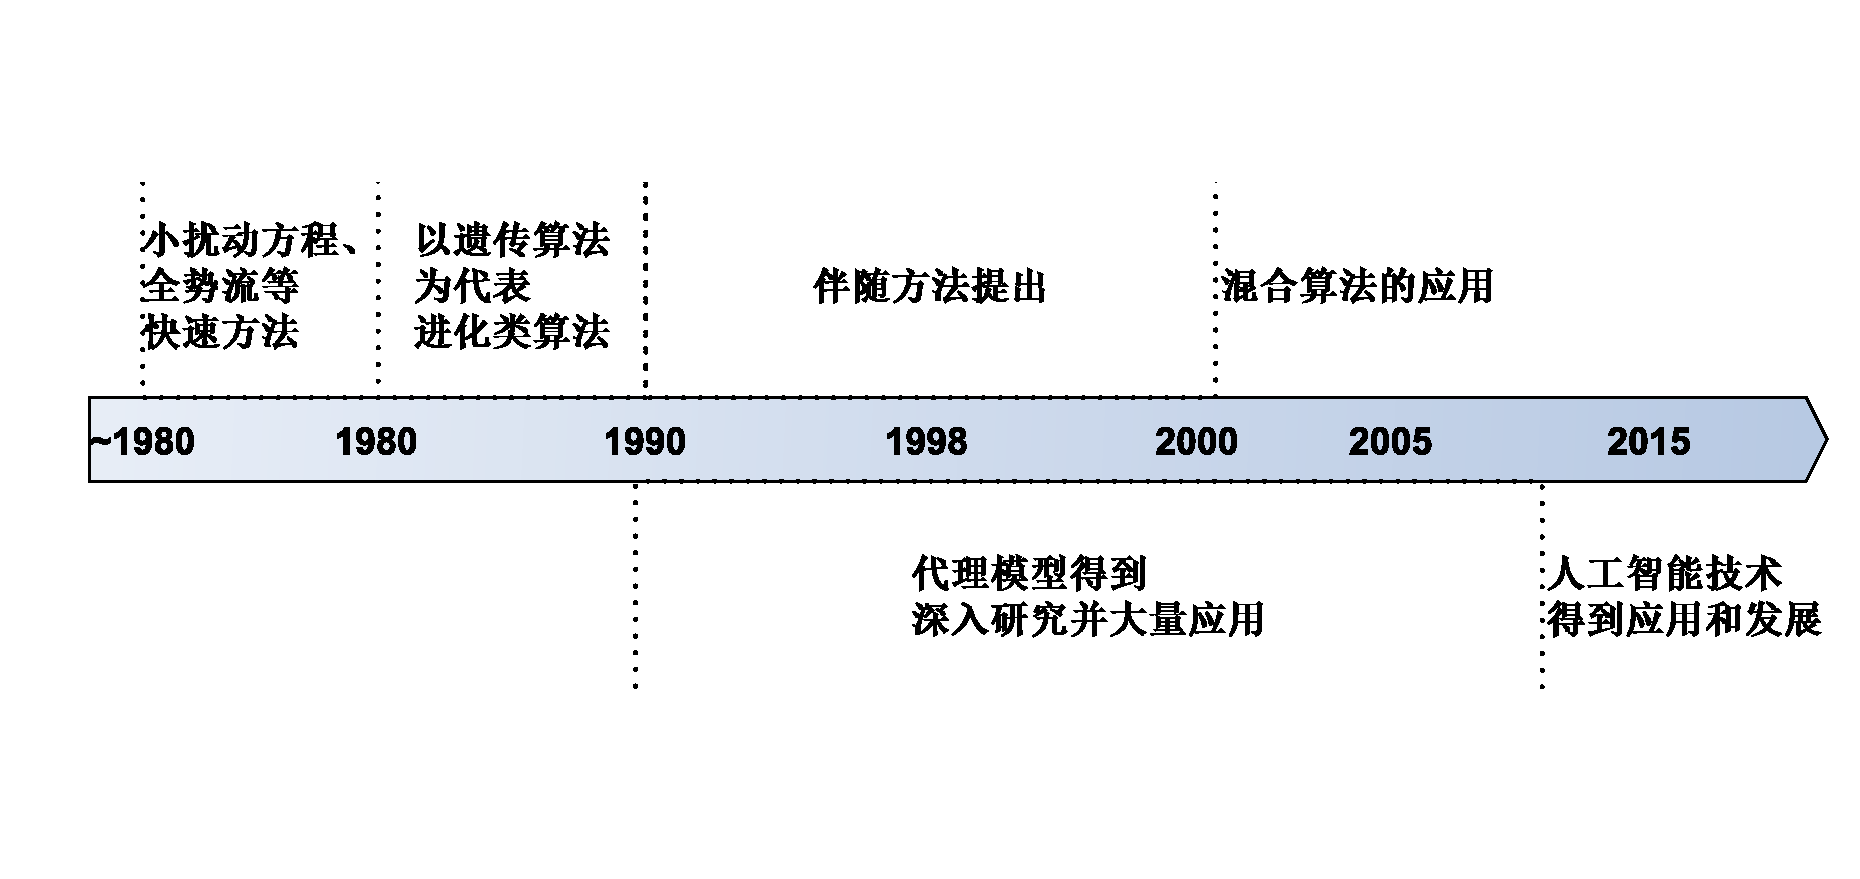
\includegraphics[width=0.92\textwidth]{figures/develop.pdf}
	\caption{气动优化技术的发展历程}
	\label{fig:1}
\end{figure}

随着机器学习技术和人工神经网络的发展,许多学者对以智能学习为基础的气动流场和气动性能预测方法进行了大量研究,基于智能学习的气动优化也是领域研究热点和本文关注的重点。
通过总结相关文献,本文对基于智能学习的气动优化技术和研究进行了整理和分类。
如图\ref{fig:智能优化}所示,基于智能学习的气动优化技术概括而言主要有两种:
一是利用传统机器学习方法和技术构建优化器、代理模型、降阶模型来减少计算开销,采用数据驱动方式,
通过对大量训练样例的“学习”构建数据间内部关系的模型,对未知数据进行预测;
二是基于深度学习方法和技术对气动特性和气动性能进行预测,利用深度神经网络强大的归纳学习能力,
提取高维、时空相关流场数据中的重要信息,构建气动流场、气动性能快速预测模型。

\begin{figure}[htp]
	\centering
	%\includegraphics[width=0.42\textwidth]{data/MLP.pdf}
	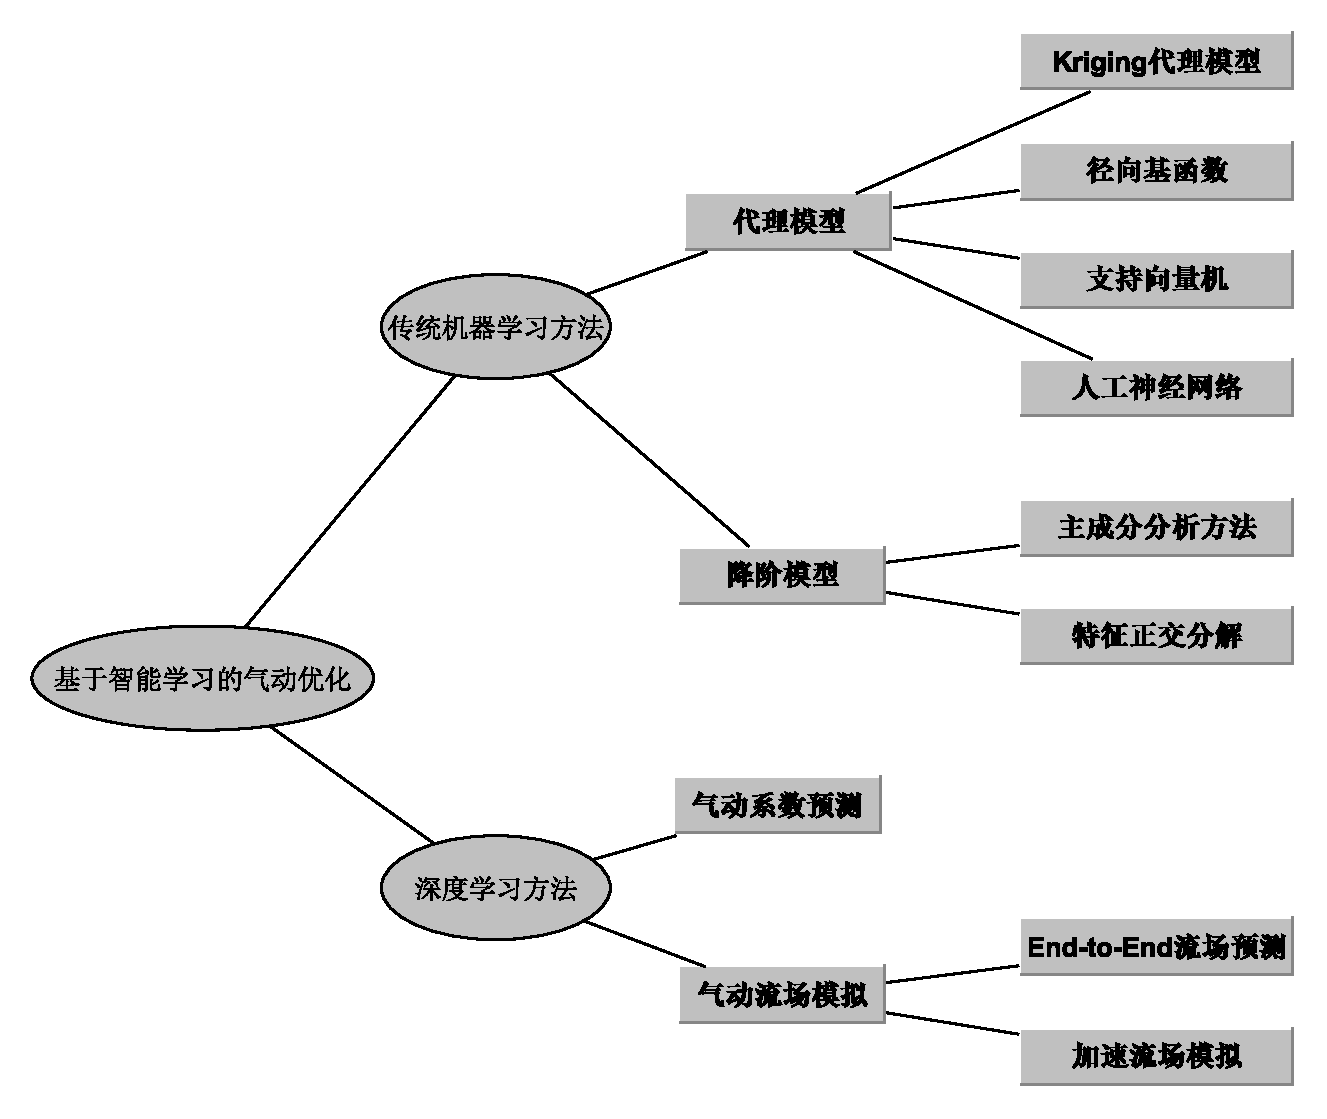
\includegraphics[width=0.92\textwidth]{figures/aicfd.pdf}
	\caption{基于智能学习的气动优化技术}
	\label{fig:智能优化}
\end{figure}

\subsection{基于传统机器学习的气动优化}
传统机器学习方法在气动优化中最典型的应用就是基于响应面法(response surface methodology,RSM)、多项式回归函数(Polynomial Regression,PR)、径向基函数(Radial Basis Functions,RBF)和人工神经网络(Artificial Neural Networks,ANN)等方法构建模型,快速从已计算的样本中预测设定的目标函数,从而达到代替CFD数值模拟的效果。此类优化方法通常被称为基于代理模型的优化方法。

Kanazaki和Tanaka等人\cite{Kanazaki2007Multi}针对飞机降落和接近失速条件下机翼升力系统的设计和优化问题,首先利用基于雷诺平均Navier-Stokes的CFD方法获取训练样本,设计了基于克里格(Kriging)代理模型的最大化升力系数的目标函数,实验结果表明相对于传统的遗传算法克里格模型显著降低了计算开销,同时实现了更好的性能。此外,作者还利用数据挖掘中的方差泛函分析方法分析了影响升力系统设计的主要因素。

张彬乾和罗烈等人\cite{张罗}针对飞翼布局设计中气动与隐身设计矛盾更为突出的问题,采用高精度气动和隐身计算方法,利用RBF神经网络代替复杂目标函数的评估,结合遗传算法和松散式代理模型管理方法,建立了翼型多目标优化设计平台。实验结果证明基于RBF神经网络的代理模型能有效模拟和评估翼型等几何形状与气动和隐身特性之间存在的强烈非线性关系。

Ju和Zhang等人\cite{Ame}为了解决蒙特卡罗模拟方法耗时长、计算开销大的问题,深入比较了人工神经网络、径向基函数和支持向量机模型(Support Vector Machine,SVM)的拟合精度,结果表明SVM精度较高,并以此基于SVM、遗传算法和蒙特卡罗方法针对翼型表面粗糙度的不确定性对翼型升阻系数进行了鲁棒性优化,实验结果表明,遗传算法-支持向量回归模型可以很好地捕获从表面粗糙度到机翼气动性能的不确定性传播。

基于代理模型的方法主要关注在给定输入数据的条件下,模型预测结果的准确性。
当研究输入变量之间的关系或者代理模型难以处理高维数据时,往往需要借助以主成分分析( Principal Component Analysis,PCA )和特征向量分解( Poper Orthogonal Decomposition,POD )为代表的机器学习方法。
比如,Kapsoulis和Dimitrios等人\cite{Kapsoulis2018Evolutionary}针对气动优化中维数灾难问题,整合进遗传算法和PCA方法,
在交叉和变异阶段使用PCA对设计变量进行降维,在降低优化复杂度的同时促使新个体的变化方向
沿着方差最大的方向进行,以提高优化效率。
此外,PCA和POD还可以用来对偏微分方程组进行降阶,得到降阶模型,再结合基于代理模型的方法,直接对气动流场进行预测。

\subsection{基于深度学习的气动优化}
近年来,以深度学习为代表的人工智能技术取得了令人瞩目的发展和成就,
深度学习等智能方法、技术也为快速、精确气动评估提供了新手段。
根据气动优化的目标不同,可以将基于深度学习的气动优化技术分为气动系数预测技术和气动流场模拟技术。
气动系数预测技术利用深度神经网络对感兴趣的气动系数(比如飞行器升力系数,升阻比等)进行回归预测,不关心流体在流场中运动的细节,属于深度学习在气动优化中的浅层运用。

Zhang和Sun等人\cite{LiftCoefficient}探讨了卷积神经网络技术的适应性以实现空气动力学元建模任务。
针对可变的流动条件和物体的几何形状,即具有多种形状的翼型,具有多个流动马赫数,雷诺数和攻角的流动条件,
训练了多个卷积神经网络以预测机翼的升力系数。
证明利用深度学习对空气动力学任务进行元建模的有效性。
将卷积神经网络结果与多层感知机的结果进行比较,发现基于卷积神经网络的元建模方法与多层感知机在学习能力方面具有可比性;
更重要的是,在几何表示约束最小的条件下,卷积神经网络模型预测准确性更高。

陈海和钱炜祺等人\cite{陈海2018}提出了一种基于深度学习的翼型气动系数预测方法,有效克服了以往方法依赖翼型设计参数以及算法复杂度随预测精度的提高呈指数级增长等缺点。该方法能够在只给出翼型图像的基础上,使用深度卷积神经网络根据翼型图像对其气动力系数进行了建模。研究结果表明显示模型预测的翼型气动系数获得了较高的精度,说明深度学习在翼型气动系数预测方面具有很好的应用前景。

利用深度学习技术对气动流场进行模拟,研究者可以观察到物理量(比如速度和压力)在流场中的分布,
获取更多有用的信息,对飞行器设计等工作进行针对性的优化和调整。
本文进一步对基于深度学习的流场模拟进行了分类:基于深度学习的流场预测方法和基于深度学习的流场模拟加速方法。
前者使用深度学习技术全部取代CFD过程实现End-to-End(端到端)流场预测,后者将深度学习方法作为加速模块并与传统的CFD求解器进行融合。

在基于深度学习的流场预测方法中,除了在神经网络模型训练阶段,需要利用CFD求解器准备训练数据以外,在模型训练完成后,推理过程不再依赖CFD方法,深度学习模型可以独立地对给定的几何体和流场条件进行预测。近年来,在基于深度学习的流场预测方向涌现了大量工作。

惠心雨和袁泽龙等人\cite{惠心雨2019}为了克服传统CFD计算需要耗费大量的计算时间与成本的缺陷,提出了一种基于深度学习的非定常周期性流场的预测框架,可以实时生成给定状态的高可信度的流场结果。将条件生成对抗网络(Generative Adversarial Networks,GAN)与卷积神经网络相结合,改进条件生成对抗网络对生成样本的约束方法,建立了基于深度学习策略采用改进的回归生成对抗网络模型,并与常规的条件生成对抗网络模型的预测结果进行对比。研究表明,基于改进的回归生成对抗网络的深度学习策略能准确预测出指定时刻的流场变量,且总时长比CFD数值模拟减少至少1个量级。

Guo和Li等人\cite{DBLP:conf/kdd/GuoLI16}针对非一致稳态层流流动建立了基于卷积神经网络(Convolutional Neural Network,CNN)的预测模型,其深度网络架构中包含了卷积编码和卷积解码(Encoder-Decoder)两部分,采用基于笛卡尔网格计算得到的符号距离函数(Signed Distance Function,SDF)作为输入,以LBM(Lattice Boltzmann Methods)求解器的模拟结果(速度场)作为训练样本标签。相对于基于二进制的几何外形表示,SDF值不仅提供了局部几何外形细节,同时包含了全局几何结构的丰富信息。作者针对二维简单形状、包含三维球体和圆柱的管道流等算例速度场进行了训练和预测,获得了较高的精度。深度神经网络预测耗时较GPU平台上LBM模拟快了2个数量级,较CPU平台上LBM模拟则快了4个数量级。该方法可以在早期设计阶段设计迭代中提供快速反馈,为构建实时、交互式设计优化空间探索提供了可能。

在Guo和Li等人的研究基础上,Bhatnagar和Afshar等人\cite{bhatnagar2019prediction}进行了改进,采用类似的深度神经网络架构,以3个翼型、4个雷诺数、21个攻角构成的RANS模拟结果作为训练数据,预测未知翼型、雷诺数、攻角的测试算例的速度场和压力场。与Guo等人的研究不同的是,作者在训练输入中增加了雷诺数、攻角信息( 在深度神经网络的全连接层处输入),且在损失函数中引入了gradient sharpening和L1正则化,提高了模型泛化能力和预测精度。

Miyanawala和Jaiman\cite{2017An}使用CNN预测了不同的阻流体的低雷诺数下的阻流体的空气动力系数。 他们提出了一种使用CNN和随机梯度下降法的数据驱动方法,用于在非定常流动问题中对Navier-Stokes方程进行模型简化。

Lee和You等人\cite{lee2019data}使用深度学习技术对在未获知的雷诺数条件下非定常圆柱绕进行了流场预测,考虑到守恒律对预测性能的影响,评测了GAN和multi-scale CNN等四种深度神经网络的预测效果。实验结果表明,对于短期预测,四种神经网络都实现了较好的预测效果;对于长期预测,考虑物理守恒的GAN和multi-scale CNN相较于不考虑物理守恒的multi-scale CNN实现了更好的性能,不考虑物理守恒的GAN实现了在四种深度神经网络中表现最好。该结果证明GAN深度神经网络充分利用了无监督训练,因此它们可以应用于先验未知的基础物理学的问题。

Filipe和Thomas等人\cite{2020Combining}使用图神经网格对流场进行了预测。基于图神经网络的方法利用网格点之间的拓扑信息和网格点上的特征向量作为输入,训练得到基于网格点的流场(包括速度场和压力场)。此外,该方法还采用粗网格上采样的结果作为输入,引入可导的求解器对粗网格点进行调整,增加了模型的泛化能力。

因为在进行预测时不需要进行耗时的迭代计算,流场预测方法的显著特点是预测效率非常高,但是预测结果的有效性即满足流体运动的规律往往难以得到保证。许多研究者针对基于深度学习的预测结果有效性进行了探索。

Ling和Templeton等人\cite{invariance}针对雷诺平均湍流模型提出了一种基于深度神经网络预测模型TBNN。
该架构使用具有不变张量的乘法层来实现将伽利略不变性嵌入预测的雷诺应力张量。 
实验结果证明了这种神经与通用神经网络相比,预测结果的准确性和物理一致性得到了提升。

Wang和Kashinath\cite{DBLP:journals/nips2019}等人提出了一种新颖的混合深度学习模型TF-Net,该模型将表示学习和湍流仿真技术相结合。TF-Net利用湍流的多尺度行为来设计可训练的尺度分离算子,以分别对不同尺度范围进行建模。 我们提供了TF-Net和基线的详尽比较,并观察到了预测误差和所需物理量(包括散度,
湍流动能和能谱)。采用不同的评估指标来评估深度深度学习模型对物理系统的预测性能包括准确性和物理一致性。


在基于深度学习的流场模拟加速方法中,传统的CFD求解器仍然参与流场模拟的过程,通过使用深度学习模型减少迭代计算量,达到计算流场模拟的效果。
相较于流场预测方法,流场模拟加速方法的模拟效率会有所下降,但是由于CFD求解器参与了流场模拟并且输出了最终了模拟结果,
使得流场模拟结果的有效性得到了充分的保证。具有代表性的工作是文献\cite{cfdnet},
Octavi和Abhinav等人针对流场模拟提出了一种基于深度学习的加速器CFDnet。将稳态流场模拟分为三个部分:基于CFD求解器的warmup,
基于深度学习模型的Inference,基于CFD求解器的Refinement。
在CFD迭代计算过程中初始阶段和最终阶段之间,利用深度神经网络建立映射代替大部分“invalid”迭代计算。
在内插数据集和外推数据集上对CFDnet的效果进行了测试,结果表明,CFDNet满足特定领域物理求解器的收敛约束,同时在层流和湍流模拟方面可达到1.9-7.4x的加速比。 此外,通过测试CFDNet对训练期间看不见的新几何形状的预测来证明其泛化能力。在这种情况下,CFDnet满足CFD求解器的收敛标准,同时收敛速度仍明显优于仅使用传统CFD求解器的对照组。


综上所述,相较于传统机器学习方法,基于深度学习的气动特性和气动性能预测具有以下优势:
1)深度模型可以自适应提取输入特征,无需进行人工筛选和精简,可极大地减少设计变量数目限制。2)深度学习很好地保留了坐标点间的空间相邻关系,其特征提取过程具有空间上的平移不变性和缩放不变性。3)深度学习由于能够提取更深层次的特征,因而拥有更强大的归纳能力,不仅可以获得气动性能预测,还可以将流场特征(如压力分布等)作为预测输出。
但是,使用深度学习技术解决气动流场优化问题,不能是简单的迁移运用,需要根据应用场景的不同,在流场模拟效率、模拟结果精度和有效性等方面进行优化,又快又好地解决气动优化问题。

\section{主要工作和创新点}
本文在深入分析现有基于智能学习的气动优化技术的基础上,受到深度卷积网络和图神经网络在计算机视觉领域成功应用的启发,将其引入来提升气动评估的效率。
本文侧重对稳态流动(即达到稳定状态后,流体中压力,速度等物理量都不随时间变化)问题的研究,
针对现有工作将深度学习技术应用到气动优化领域的一些不足,在流场数据表示,网络架构搭建与优化,嵌入物理模型约束和性能评价指标等方面展开相关研究。本文贡献了两个测试数据集,用于测试与分析基于不同深度学习网络的气动优化方法,并得到相应结论。
总结而言,本文的主要工作和创新点如下:
\begin{itemize}
	\item[(1)] 提出了一种基于深度卷积网络(Deep Neural Networks,DNN)的气动流场预测方法。
	首先,针对深度网络的输入数据的表示问题,提出了针对流场流场数据的特征表示方法;利用基于LBM(Lattice Boltzmann Method)的数值模拟求解器构造了两种不同流动条件下的数据集;
	其次,基于图像分割领域的深度网络模型,设计了适用于流场预测的网络架构,同时引入了注意力机制和神经网络剪枝技术,分别对模型的预测精度和推理速度进行了优化;
	研究流体流动的特性,基于质量守恒和动量守恒的控制方程,设计了嵌入物理模型约束的损失函数。
	在性能评价指标方面,除了深度学习训练常用的相对评价误差以外,本文提出了新的评价指标用来评估气动预测模型在感兴趣区域(Region of  interest,RoI)和物理守恒性等方面的预测效果。
	实验结果表明该方法能够对给定的输入数据进行快速的预测,相较于LBM求解器预测速度提升了四个数量级,同时保证预测误差低于5\%。
		
	
	\item[(2)] 提出了一种基于图神经网络(Graph Neural  Networks,GNN)的气动模拟加速方法。
	首先,利用网格生成软件生成的网格文件,基于算例的边界条件设置,构造了带有拓扑信息和节点特征信息的图结构输入数据,用于训练图神经网络;
	其次,利用图卷积网络(Graph  Convolutional Network,GCN)构建气动模拟的加速模块。
	完成模型训练后,将模型的推理结果反馈给CFD求解器,为求解器迭代计算过程提供一个更接近于稳定状态的初场,减少CFD的模拟时间。
	实验结果表明,基于GNN的气动模拟加速方法能够有效提升流场模拟的效率,此外,通过CFD求解器对GCN的模拟结果进行优化,保证了模拟结果的预测一致性。
	
	
	
\end{itemize}

\section{论文结构}
本文主要研究基于深度学习方法和技术的气动流场模拟方法,利用深度神经网络和图神经网络设计实现了气动流场的预测方法和模拟加速方法,论文的主要结构如下:

第一章:主要介绍了传统CFD模拟在实际工程应用中遇到的挑战,智能学习方法和技术在气动优化方向的研究现状以及论文的主要工作。

第二章:通过分析传统CFD模拟流程定义了研究问题,介绍了计算流体力学相关理论基础;针对第三章、第四章研究内容,
重点介绍了相关的深度学习知识与技术,包括常用的深度卷积网络模型和图神经网络模型。

第三章:介绍基于深度卷积神经网络的气动流场预测方法,提出针对流场数据的表示方法。
基于图像分割网络设计气动流场预测架构,通过嵌入注意力模块和设计嵌入物理约束的损失函数对流场预测模型进行针对性的优化。
介绍利用CFD求解器生成实验数据集的流程,定义新的流场预测结果的评价指标。
通过实验和结果分析,对模型预测结果的准确率、有效性以及流场模拟效率进行了全面的评估。

第四章:介绍基于图神经网络的气动流场模拟加速方法,提出基于图结构的流场数据表示方法,
基于图卷积网络设计气动流场模拟加速模块,利用CFD求解器对模型模拟结果进行优化,
在提升流场模拟效率的同时保证流场模拟结果的有效性。
在测试集上对提出的方法进行实验论证,分析实验结果。

第五章:对本文的工作进行总结和评价,分析现有研究工作的不足和缺陷,对未来的研究方向和研究内容进行展望。












\chapter{研究基础与相关技术}

近年来,深度学习一直是计算机领域乃至多学科交叉应用领域的研究热点,不仅在计算机视觉方向有着广泛的应用,在光学、材料和航空航天等领域也出现了相关研究。尤其对于大数据应用场景,基于深度学习的方法已经成为重要的数据挖掘手段。
对于气动优化乃至整个CFD领域而言,深度学习方法在此领域获得发展并取得成功只是时间问题。
为了便于阐述本课题工作,本章首先定义了本课题要解决的问题,即明确利用深度学习方法和技术要解决的问题和要达到的效果;
其次介绍了CFD相关的基础理论,主要包括建立在宏观层次的Navier-Stokes(N-S)方程和介观层次的格子Boltzmann方法(Lattice Boltzmann Methods,LBM);最后介绍了四种与本文工作紧密相关的深度神经网络和图神经网络模型。

\section{研究问题定义}
利用传统CFD方法对流体问题(包括气动优化问题)进行研究的流程如图\ref{fig:cfdflow}所示。
\begin{figure}[htp]
	\centering
	%\includegraphics[width=0.42\textwidth]{data/MLP.pdf}
	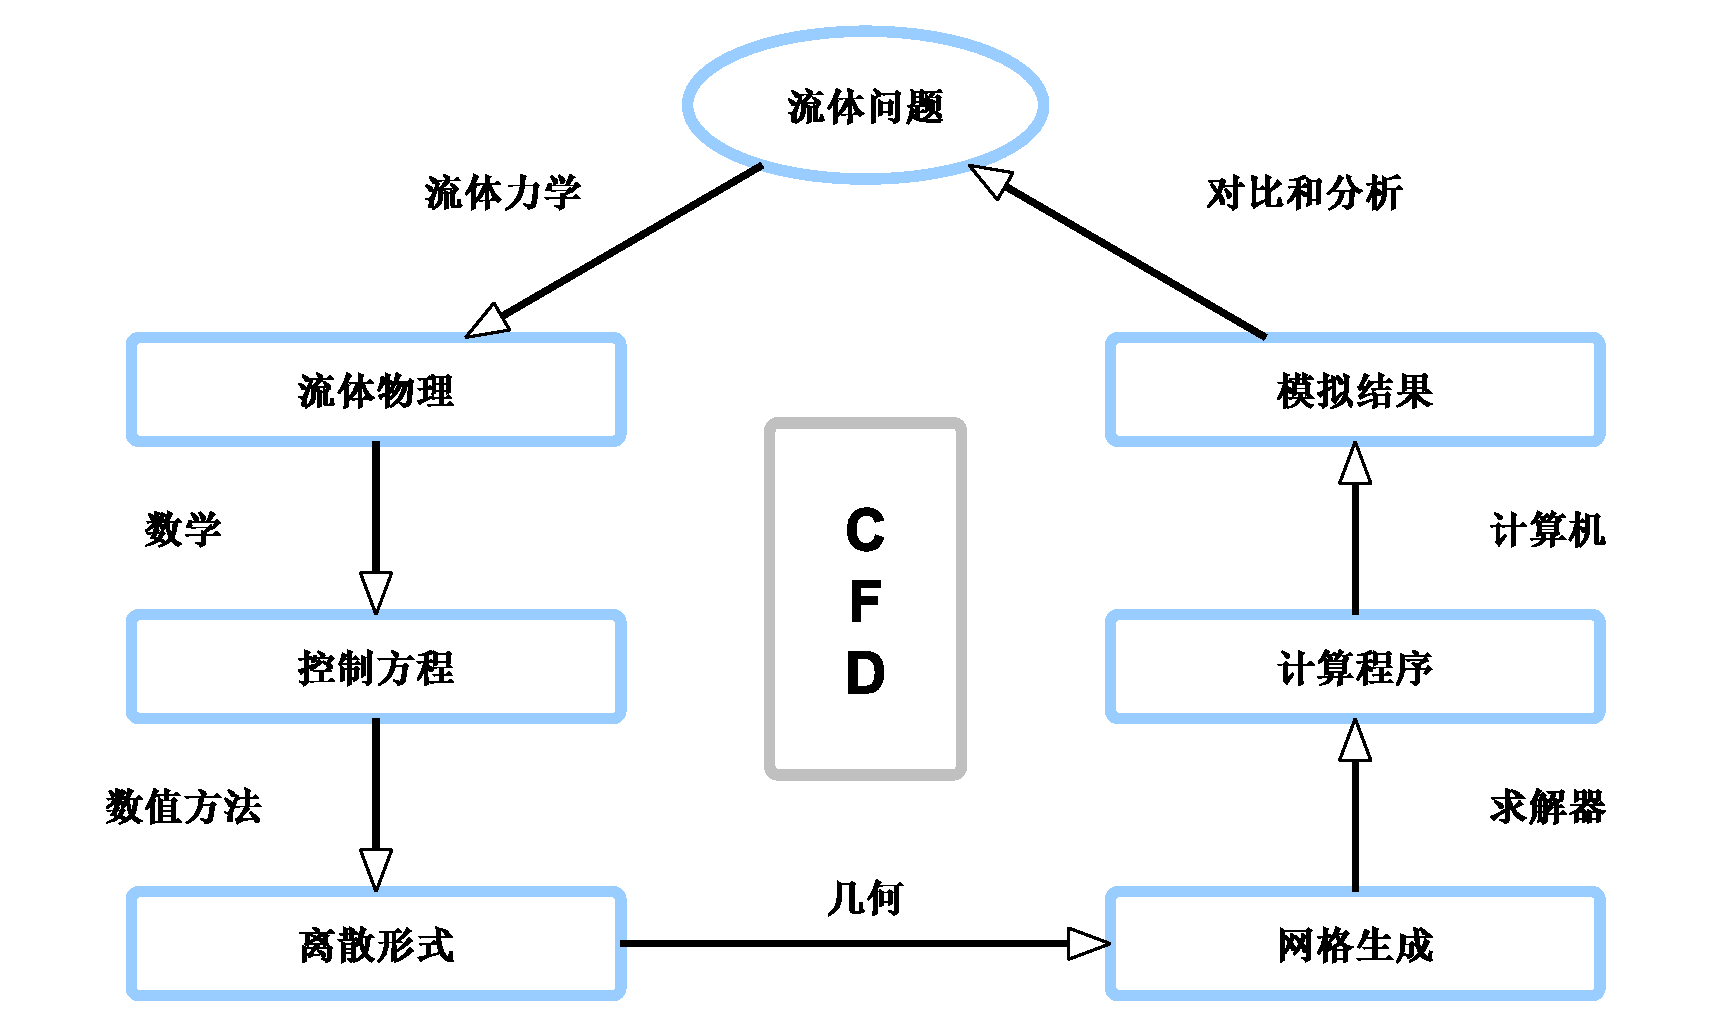
\includegraphics[width=0.92\textwidth]{figures/cfdflow.pdf}
	\caption{利用传统CFD方法研究和解决流体问题的流程示意图}
	\label{fig:cfdflow}
\end{figure}


首先利用流体力学知识对流体问题进行理论分析,建立物理模型;
根据流体运动遵循的基本规律,利用数学方法推导出流体流动的控制方程,
宏观层面上有粘性流动的Navier-Stokes方程和无粘流动的欧拉方程;
针对特定的流体问题,明确其物理基础和假设,简化控制方程、确定边界条件和初始条件。
由于CFD方法是利用数值计算对流体流动进行模拟,所以研究的不是连续运动的流体,必须利用数值方法对时间和空间进行离散,
以便进行迭代计算求解。对空间的离散方法包括有限差分方法,有限元方法和有限体积方法;
对时间的离散通常包括适用于定常流体问题求解的显示方法和适用于非定常问题的求解的隐式方法。
确定离散形式之后,需要对几何进行划分,即生成网络,在网格上对控制方程进行求解。
网格生成之后,选择合适的CFD求解器,依据初始条件和边界条件对求解器的参数进行设置,
最后利用计算机进行迭代计算至模拟结果收敛。



这种全阶CFD模拟往往耗时较长,难以满足全面、快速的设计空间探索需求。
为了加速CFD模拟进程,提升气动优化效率,本文针对二维稳态流动问题,
提出了两种基于深度学习的气动优化模型,图\ref{fig:cfd_dnnflow}展示了这两种模型的工作流程。

\begin{figure}[htp]
	\centering
	%\includegraphics[width=0.42\textwidth]{data/MLP.pdf}
	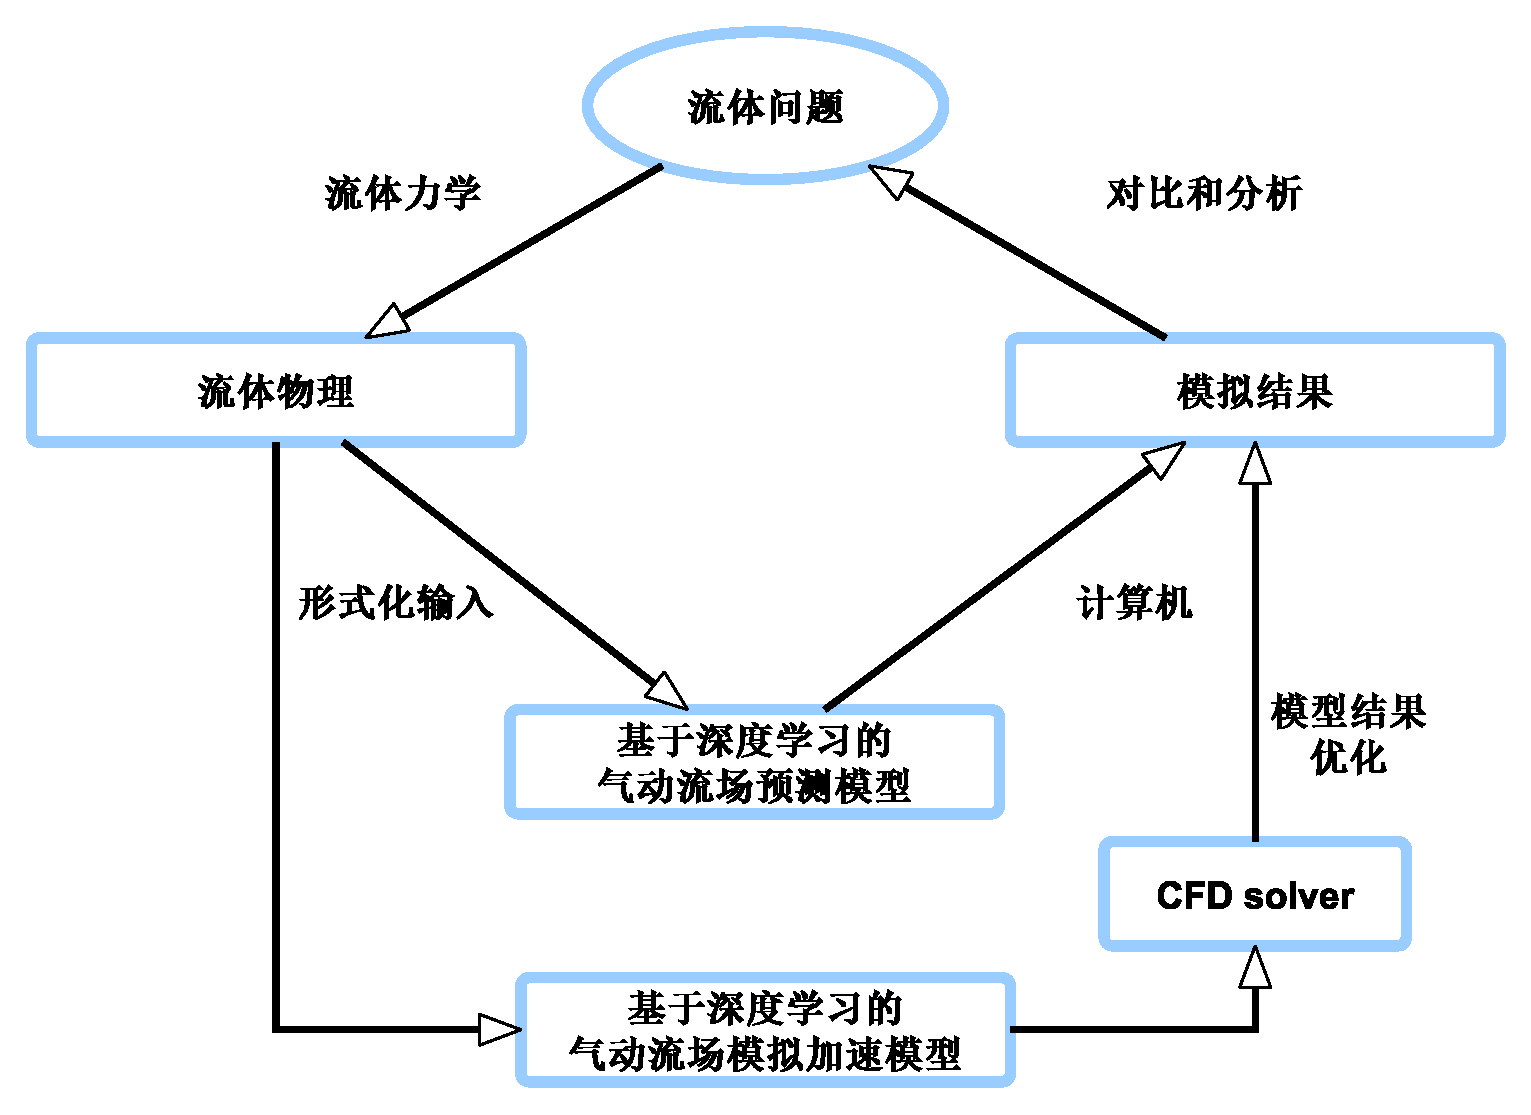
\includegraphics[width=0.92\textwidth]{figures/cfd_dnnflow.pdf}
	\caption{基于深度学习的气动优化模型工作流程示意图}
	\label{fig:cfd_dnnflow}
\end{figure}

在气动流场预测模型中,将边界条件和几何外形形式化为适合神经网络训练的输入,
利用深度学习方法构建端到端的预测模型,通过神经网络正向推理过程,得到对应的气动流场预测结果;
气动流场模拟加速模型的流程与气动流场预测模型类似,不同之处在于模型训练完成后,将深度学习模型的结果输入到CFD求解器中,为CFD求解过程提供一个更加接近收敛状态的初场,从而达到减少迭代计算量、加速模拟的效果。



\section{计算流体动力学基础理论}
根据对气体在不同尺度上动力学规律的描述,计算流体力学方法可分为三类:宏观、介观和微观。

宏观尺度上,假设流体连续地充满整个空间,流体被假设为连续介质。满足质量守恒、动量守恒以及能量守恒;在数学上,流体可由欧拉方程组、N-S方程组进行描述;在数值计算上,通过各种离散方法将欧拉方程组或N-S方程组离散成各种代数方程。
介观尺度(分子自由程尺度)上,流体被离散为一系列流体粒子;在数学上,流体由统计力学方程描述;在数值计算上,构造符合一定物理规律的演化机制,通过演化得到与物理规律相符的数值结果。
微观尺度上,不再假设流体介质为连续的,通过对每一个分子的运动进行模拟计算,
然后在采用不同的方式进行统计平均,以获得流体的宏观运动规律。因为要对每一个分子的运动进行模拟计算,微观层面的方法往往需要消耗大量的计算资源。
根据与本文研究内容的相关性,本节重点介绍格子Boltzmann方法和雷诺平均N-S方程。



\subsection{格子Boltzmann方法的基本原理}

\subsubsection{BGK模型}
Boltzmann方程的基本思想是
在任何一个宏观系统中,每一个分子的微观运动都遵循力学规律,因此只要算出大量分子的个别运动就可以确定系统的宏观参数;
求出每一分子处于某种状态下的概率,通过统计的方法得出系统的宏观参数。 
基于以上思想,物理学家 Boltzmann提出方程的三大假设:
\begin{itemize}
	\item[(1)] 分子相互碰撞只考虑二体碰撞,认为3个及3个以上分子碰撞的概率很小;
	\item[(2)] 各个分子的速度分布是不依赖于另外的分子而独立存在;
	\item[(3)] 外力不影响局部碰撞的动力学行为。 	
\end{itemize}

定义速度分布函数$f$是空间位置矢量$\vec{r}$,分子速度矢量$\vec{\xi}$以及时间$t$的函数。根据$f$的定义有:
\begin{equation}n=\int f(\vec{r}, \vec{\xi}, t) d \xi\end{equation}
\noindent n即为t时刻,$\vec{r}$处单位体积内的分子数。
根据假设,速度分布函数$f$可由两项引起改变,第一项是分子的运动,第二项是分子的碰撞,
先考虑没有碰撞的情况,$m \vec{a}$为作用在每个分子上的外力,m是分子质量,
任意分子,如果在时间间隔$d t$内无碰撞,则分子位置由$\vec{r}$变为$\vec{r}+d \vec{r}$,
速度变为$\vec{\xi}+\vec{a} d t$,则原t时刻,在$d \vec{r} d \vec{\xi}$中的气体分子全部转移到$\vec{r}+d \vec{r}$,$\vec{\xi}+\vec{a} d t$的$d \vec{r} d \vec{\xi}$中,即有
\begin{equation}f(\vec{r}+d \vec{r}, \vec{\xi}+\vec{a} d t, t+d t) d \vec{r} d \vec{\xi}=f(\vec{r}, \vec{\xi}, t) d \vec{r} d \vec{\xi}\end{equation}

\noindent 在$(\vec{r}, \vec{\xi}, t)$处进行Taylor展开,化简有分子的运动对速度分布函数f的影响:

\begin{equation}
\label{运动}
\left(\frac{\partial f}{\partial t}\right)_{\text {运动 }}=-\vec{\xi} \cdot \frac{\partial f}{\partial \vec{r}}-\vec{a} \cdot \frac{\partial f}{\partial \vec{\xi}}\end{equation}

\noindent 考虑分子间的碰撞,应用刚体碰撞模型,根据碰撞前后动量守恒和能量守恒可得碰撞对速度分布函数的影响:

\begin{equation}
\label{碰撞}
\left(\frac{\partial f_{1}}{\partial t}\right)_{\text {碰撞 }}=\iint\left(f_{1}^{\prime} f_{2}^{\prime}-f_{1} f_{2}\right) d_{D}^{2}|\vec{g}| \cos \theta d \Omega d \vec{\xi}_{2}\end{equation}

\noindent  其中$\vec{g} =  f_{1} - f_{2}$, $f_{1}$,$f_{2}$为碰撞前分子速度,$f_{1}^{\prime}$,$f_{2}^{\prime}$是碰撞后分子速度;$d_{D}$是分子直径,
$d \Omega$表示球面微元在第一个分子的固定角。

综合公式\ref{运动}和\ref{碰撞}有:
\begin{equation}\left(\frac{\partial f}{\partial t}\right)=\left(\frac{\partial f}{\partial t}\right)_{\text {运动 }}+\left(\frac{\partial f}{\partial t}\right)_{\text {碰撞 }}\end{equation}

\noindent 化简即有:
\begin{equation}
\label{Boltzmann方程}
\left(\frac{\partial f}{\partial t}\right)+\vec{\xi} \cdot \frac{\partial f}{\partial \vec{r}}+\vec{a} \cdot \frac{\partial f}{\partial \vec{\xi}}=\iint\left(f_{1}^{\prime} f_{2}^{\prime}-f_{1} f_{2}\right) d_{D}^{2}|\vec{g}| \cos \theta d \Omega d \vec{\xi}_{1}\end{equation}

由于碰撞项计算涉及复杂的非线性积分,所以Boltzmann方程难以求解。因此,Bhatnagar,Gross和Krook提出使用一个简单的算子$\Omega_{f}$替代方程\ref{Boltzmann方程}右边碰撞项,称为BGK近似模型。
最简单的算子可以认为碰撞使f趋于平衡分布$f^{e q}$。设改变率与$\left(f^{e q}-f\right)$成正比,系数为$\nu$,为碰撞频率即弛豫时间的导数${1}/{\tau_{0}}$,则Boltzmann方程简化为:

\begin{equation}\left(\frac{\partial f}{\partial t}\right)+\vec{\xi} \cdot \frac{\partial f}{\partial \vec{r}}+\vec{a} \cdot \frac{\partial f}{\partial \vec{\xi}}=v\left[f^{e q}(\vec{r}, \vec{\xi}, t)-f(\vec{r}, \vec{\xi}, t)\right]\end{equation}

\noindent 等式右边即为线性算子$\Omega_{f}$。

\subsubsection{格子Boltzmann方程}
格子Boltzmann方程是BGK方程的进一步离散形式,这一离散形式包括了速度离散、时间离散、空间离散。
对于时间离散,由于微观粒子时刻在做无规则的热运动,因此微观粒子的速度是连续的,其速度方向和大小有无穷个,但粒子的运动并不会显著影响流体的宏观运动。
因此可以将分子速度简化为有限维速度空间,$\left\{\overrightarrow{e_{0}}, \vec{e}_{1}, \ldots, \overrightarrow{e_{N}}\right\}$,N表示速度种类数。
连续的速度分布函数f也被相应离散为$\left\{f_{0}, f_{1}, \ldots, f_{N}\right\}$,
其中$f_{\alpha}=f_{\alpha}\left(\vec{r}, \overrightarrow{e_{\alpha}}, t\right)$,
$\alpha=0,1, \ldots, N$。于是可得离散的Boltzmann方程:

\begin{equation}
\label{速度离散}
\frac{\partial f_{\alpha}}{\partial t}+\overrightarrow{e_{\alpha}} \cdot \nabla f_{\alpha}=-\frac{1}{\tau_{0}}\left(f_{\alpha}-f_{\alpha}^{e q}\right)+F_{\alpha}\end{equation}

\noindent 其中$f_{\alpha}^{e q}$分子局部平衡分布;$F_{\alpha}$为离散速度空间的外力项。
在速度离散的基础上,进一步进行时间离散和空间离散,对公式\ref{速度离散}积分,采用矩形法对公式右边项进行逼近有:

\begin{equation}
\label{LBM方程}
f_{\alpha}\left(\vec{r}+\overrightarrow{e_{\alpha}} \delta_{t}, t+\delta_{t}\right)-f_{\alpha}(\vec{r}, t)=-\frac{1}{\tau}\left[f_{\alpha}(\vec{r}, t)-f_{\alpha}^{e q}(\vec{r}, t)\right]+\delta_{t} F_{\alpha}(\vec{r}, t)\end{equation}

方程\ref{LBM方程}即为格子Boltzmann方程。
DnQm模型\cite{Y1992Lattice}是格子Boltzmann方程基本模型,n表示空间维数,m表示速度的类型,常见的有D2Q7模型、D2Q9模型、D3Q15模型和D3Q19模型等,图\ref{fig:dnqm}给出了D2Q9和D3Q19的示意图。


\begin{figure}[htb]
	\centering
	\subfloat[D2Q9]{\label{fig:d2q9}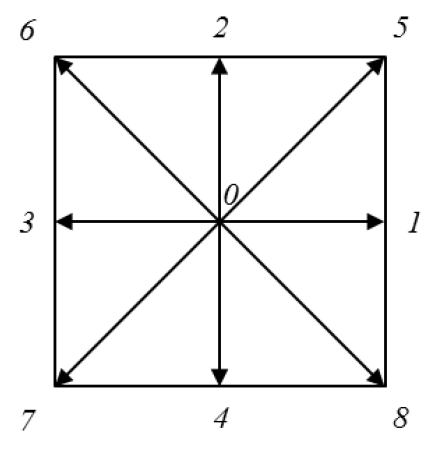
\includegraphics[width=0.35\textwidth]{figures/d2q9.png}} \qquad
	\subfloat[D3Q19]{\label{fig:d3q19}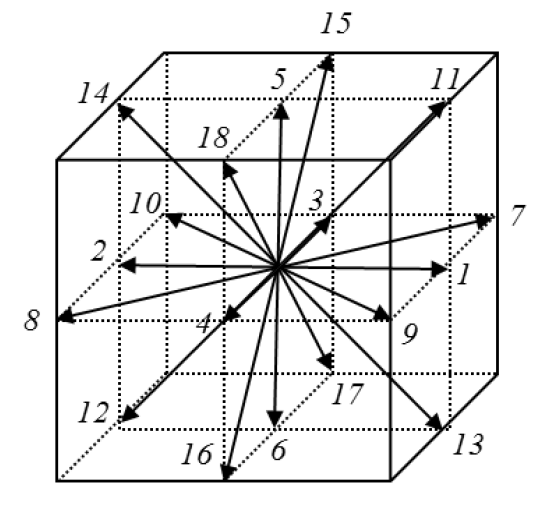
\includegraphics[width=0.38\textwidth]{figures/d3q19.png}} 
	\caption{D2Q9模型和D3Q19模型速度离散示意图}
	\label{fig:dnqm}
\end{figure}

\noindent D2Q9模型适用于二维流动问题,将速度根据大小和方向的不同分为了9类;
D3Q19模型适用于三维流动问题,速度离散也更加复杂,将速度根据大小和方向的不同分为了19类。

LBM方法相对于宏观方法具有精度高的特点,与传统方法相比,对流项(碰撞项)是线性的,算法简单;由于粒子的运动只有碰撞和迁移,LBM方法编程容易;
此外,LBM运算具有局部性,每个粒子只与周围相邻粒子有关,局部运算可同步进行,适合并行计算。
因为以上优点,LBM方法在CFD领域应用广泛,利用深度学习技术提升LBM方法的模拟效率具有重要意义。


\subsection{雷诺平均N-S(RANS)方程}
流体流动一般由以下三个基本定律来控制:
(1)质量守恒定律;(2)牛顿第二定律;(3)能量守恒定律。基于这三个基本的物理学定理构建的流动模型,将导出一组控制方程,比如适合粘性流动的Navier-Stokes方程(N-S方程)。

流体流动有不同的流动状态,当流速很小时,流体分层流动,互不混合,称为层流;当流速逐渐增大,流体的流线开始出现波浪状的摆动,摆动的频率及振幅随流速的增加而增加,此种流况称为过渡流;当流速增加到很大时,流线不再清楚可辨,流场中有许多小漩涡,层流被破坏,相邻流层间出现滑动和混合,这时的流体作不规则运动,这种运动称为湍流。

湍流运动过程十分复杂,在数学上表现出极高的非线性,使用数值模拟方法解决湍流一直是流体力学研究的难点。
虽然N-S方程能够准确地描述湍流运动的细节,但求解这样一个复杂的方程会花费大量的精力和时间。

目前在CFD领域,解决湍流问题的方法主要包括直接数值模拟(Direct numerical simulation,
DNS)、大涡模拟(Large eddy simulation,LES)和雷诺平均( Reynold average Navier-Stokes,RANS)。
其中DNS和LES对网格精细度要求较高,在工程应用上还处于尚不成熟的阶段。
为了在精度和效率上满足实际工程需要,研究者提出了基于时均理论的雷诺平均N-S模型,RANS在工程上应用也最多。
对于本文研究的稳态不可压流动,在笛卡尔坐标系下有,连续性方程:

\begin{equation}
\label{连续性方程}
\frac{\partial \rho}{\partial t}+\frac{\partial(\rho u)}{\partial x}+\frac{\partial(\rho v)}{\partial y}+\frac{\partial(\rho w)}{\partial z}=0\end{equation}

\noindent 对动量方程采用二阶迎风对流格式离散:


\begin{equation}\begin{array}{c}
\label{动量方程}
u \frac{\partial u}{\partial x}+v \frac{\partial u}{\partial y}+w \frac{\partial u}{\partial z}=-\frac{1}{\rho} \frac{\partial p}{\partial x}+\frac{\mu}{\rho} \nabla^{2} u \\
u \frac{\partial v}{\partial x}+v \frac{\partial v}{\partial y}+w \frac{\partial v}{\partial z}=-\frac{1}{\rho} \frac{\partial p}{\partial y}+\frac{\mu}{\rho} \nabla^{2} v \\
u \frac{\partial v}{\partial x}+v \frac{\partial w}{\partial y}+w \frac{\partial w}{\partial z}=-\frac{1}{\rho} \frac{\partial p}{\partial z}+\frac{\mu}{\rho} \nabla^{2} w
\end{array}
\end{equation}


\noindent 对方程\ref{连续性方程}和\ref{动量方程}进行雷诺平均有:
\begin{equation}\frac{\partial \rho}{\partial t}+\frac{\partial}{\partial x_{i}}\left(\rho \bar{u}_{i}\right)=0\end{equation}

\begin{equation}\frac{\partial}{\partial t}\left(\rho \bar{u}_{i}\right)+\frac{\partial}{\partial x_{i}}\left(\rho \bar{u}_{j} \bar{u}_{i}\right)=-\frac{\partial \bar{p}}{\partial x_{i}}+\frac{\partial \bar{\sigma}_{i j}}{\partial x_{j}}+\frac{\partial}{\partial x_{j}}\left(-\rho \bar{u}_{i}^{\prime} \bar{u}_{j}^{\prime}\right)\end{equation}

\noindent 其中$\bar{u}_{i}$为雷诺平均速度分量,$\rho$为密度,$p$为压强,$\bar{u}_{i}^{\prime}$平均脉动速度,$\partial \bar{\sigma}_{i j}$为应力张量分量。


一般地,在对湍流流动的N-S方程平均后,得到的平均方程中会包含未知的雷诺应力项,导致了方程求解的不封闭问题。
因此需要根据湍流运动规律以寻找附加条件和关系式构建湍流模型使方程封闭。
此外,在进行雷诺平均的过程中损失了部分流动细节,引入湍流模型对于找回这些细节十分必要。
对于RANS湍流模拟,根据Boussinesq\cite{schmitt2007boussinesq}假设,粘性系数由层流部分和湍流部分构成,
即$\nu=\nu_{L}+\nu_{T}$,其中$\nu_{L}$是层流运动粘性系数(laminar kinematic viscosity), $\nu_{T}$是湍流运动粘性系数(eddy-viscosity variable),由湍流模型方程计算得到。

常用的湍流模型可根据所采用的微分方程数进行分类为:零方程模型、一方程模型、两方程模型、四方程模型、七方程模型等\cite{1998A}。本文使用的湍流模型是Spalart-Allmaras(SA)模型\cite{SAequation},
是一种主要用在航空领域的单方程湍流模型,对墙壁束缚(wall-bounded)流动,显示出很好的效果。
SA模型认为在自由剪切流中能量和信息由大尺度流动流向小尺度流动,涡粘系数只有产生项和扩散项,所以满足以下基本运输方程:

\begin{equation}
\begin{split}
\frac{D F}{D t}= & \frac{\partial F}{\partial t}+(u \cdot \nabla) F \\ = & {Diffusion} + {Production} - {Destruction}
\end{split}
\end{equation}

\noindent 其中$F$外力,\textit{diffusion}是扩散项,\textit{production}是产生项,\textit{destruction}是损失项。
对于湍流运动粘性系数$\nu_{T}$应用该运输方程有:

\begin{equation}\label{SA_equo}
\begin{split}
\frac{D \nu_{T}}{D t}=& \frac{1}{\sigma}\left[\nabla \cdot((\nu_{L}+\nu_{T}) \nabla \nu_{T})+c_{b 2}(\nabla \nu_{T})^{2}\right] +c_{b 1} \tilde{S} \nu_{T} - \\ &c_{w 1} f_{w}\left[\frac{\nu_{T}}{d}\right]^{2}
\end{split}
\end{equation}

\noindent 其中$\sigma$普朗特数,$c_{b 1}$和$c_{b 2}$为闭合常数,$d$表示到壁面的最短距离。
$\tilde{S}$可以通过$d$和速度$u$计算得到,
$f_{w}$是一个关于$\tilde{S}$和$\nu_{T}$无量纲函数,用于解决在边界层外部损失项收敛慢的问题。

虽然许多湍流模型在某些特定的应用场景取得成功,但至今仍未有一个有效的通用的湍流模型,这也直接导致了RANS缺少普适性。
本文首先基于特定流场条件,模拟生成流场数据集,然后利用深度学习方法从大量流场数据学习流场运动规律,
最后得到能够进行快速精准流场预测的代替模型。


\section{深度学习相关模型介绍}
深度学习是机器学习的重要分支,自2006年提出以来,深度学习理论和技术以及获得了长足的发展,常见的深度学习模型有深度信念网络\cite{深度信念网络},自动编码器\cite{Bengio2013Representation},卷积神经网络\cite{Lecun1998Gradient},递归神经网络\cite{Williams2014A},生成对抗网络\cite{GAN}等。
此外,深度学习在与强化学习、图网络结合方面也非常成功,比较前沿的研究领域有深度强化学习\cite{Deepreinforcementlearning}和图神经网络\cite{2016Semi}等。
深度学习的快速发展为解决气动优化提供了新的思路和方法,
利用深度学习方法提升气动优化效率的核心思想是基于神经网络构建从输入到输出的映射函数,
从而代替或者加速CFD求解器的迭代计算过程,
不同于常规的图像分类任务,深度神经网络需要在大量数据中学习到从给定输入到对应输出的表示方法。

针对流场数据中的欧式空间数据,经过类比分析,我们发现图像处理中的image-to-image\cite{DBLP:conf/miccai/RonnebergerFB15,DBLP:conf/cvpr/LongSD15,isola2017image,CycleGAN2017,DBLP:conf/cvpr/AmodioK19}的转换方法尤其适用于气动优化场景。
对于非欧式空间数据,本文引入了基于图神经网络的架构进行模型训练。
如何将流场数据处理成为深度神经网络可接受的形式将在第三章详细阐述,本节重点介绍三类用于图像回归任务的深度神经网络和图神经网络中的图卷积网络。
关于深度学习的其他基础理论知识,包括网络基础结构单元,损失函数,优化算法等,可参见文献\cite{dnnsurvey}。

\subsection{卷积自编码网络}
卷积自编码网络(Convolutional Autoencoders)是自编码网络\cite{Bengio2013Representation}的变体。
自编码网络及其变体都有类似的网络结构:编码器和解码器。
传统的自编码器是一种无监督学习算法,数据没有标签,
输入数据$X$经过编码器处理得到输入数据的特征表示z,编码结果经过解码器得到输出$X^{\prime}$,具体过程可以表示为:
\begin{equation}
z=g(X ; \phi) 
\vspace{-0.2cm}
\end{equation}
\begin{equation}
X^{\prime}=f(z ; \theta)
\end{equation}
其中$g(\bullet ; \phi)$和$f(\bullet ; \theta)$分别表示编码器和解码器,$\phi$和$\theta$是相应的参数。

损失函数一般可以定义为输入$X$和输出$X^{\prime}$的最小均方误差(Mean Squared Error,MSE):
\begin{equation}
Loss_{MSE} = \min _{\phi, \theta}\left\|X-X^{\prime}\right\|_{2}^{2}
\end{equation}

一般而言,z的维度远小于输入$X$的维度,网络通过这样编码和解码的方式,实现对输入数据的降维且尽量不损失数据信息。

但是传统的自编码器在处理图片格式数据时,由于采用了全连接操作,忽略了图像中的空间关系,数据切片和数据堆叠会导致信息大量丢失。
为了克服这一缺点,卷积自编码网络采用卷积层来构造自编码器。
图\ref{fig:CAE}是卷积自编码网络的示意图,深色部分代表编码器,通常由卷积层和池化层构成,卷积层负责信息提取,池化层负责空域下采样;
浅色部分代表解码器,由卷积层和上采样层构成,有时也利用逆卷积操作替代卷积和上采样操作进行原始信息的复原。

\begin{figure}[htp]
	\centering
	%\includegraphics[width=0.42\textwidth]{data/MLP.pdf}
	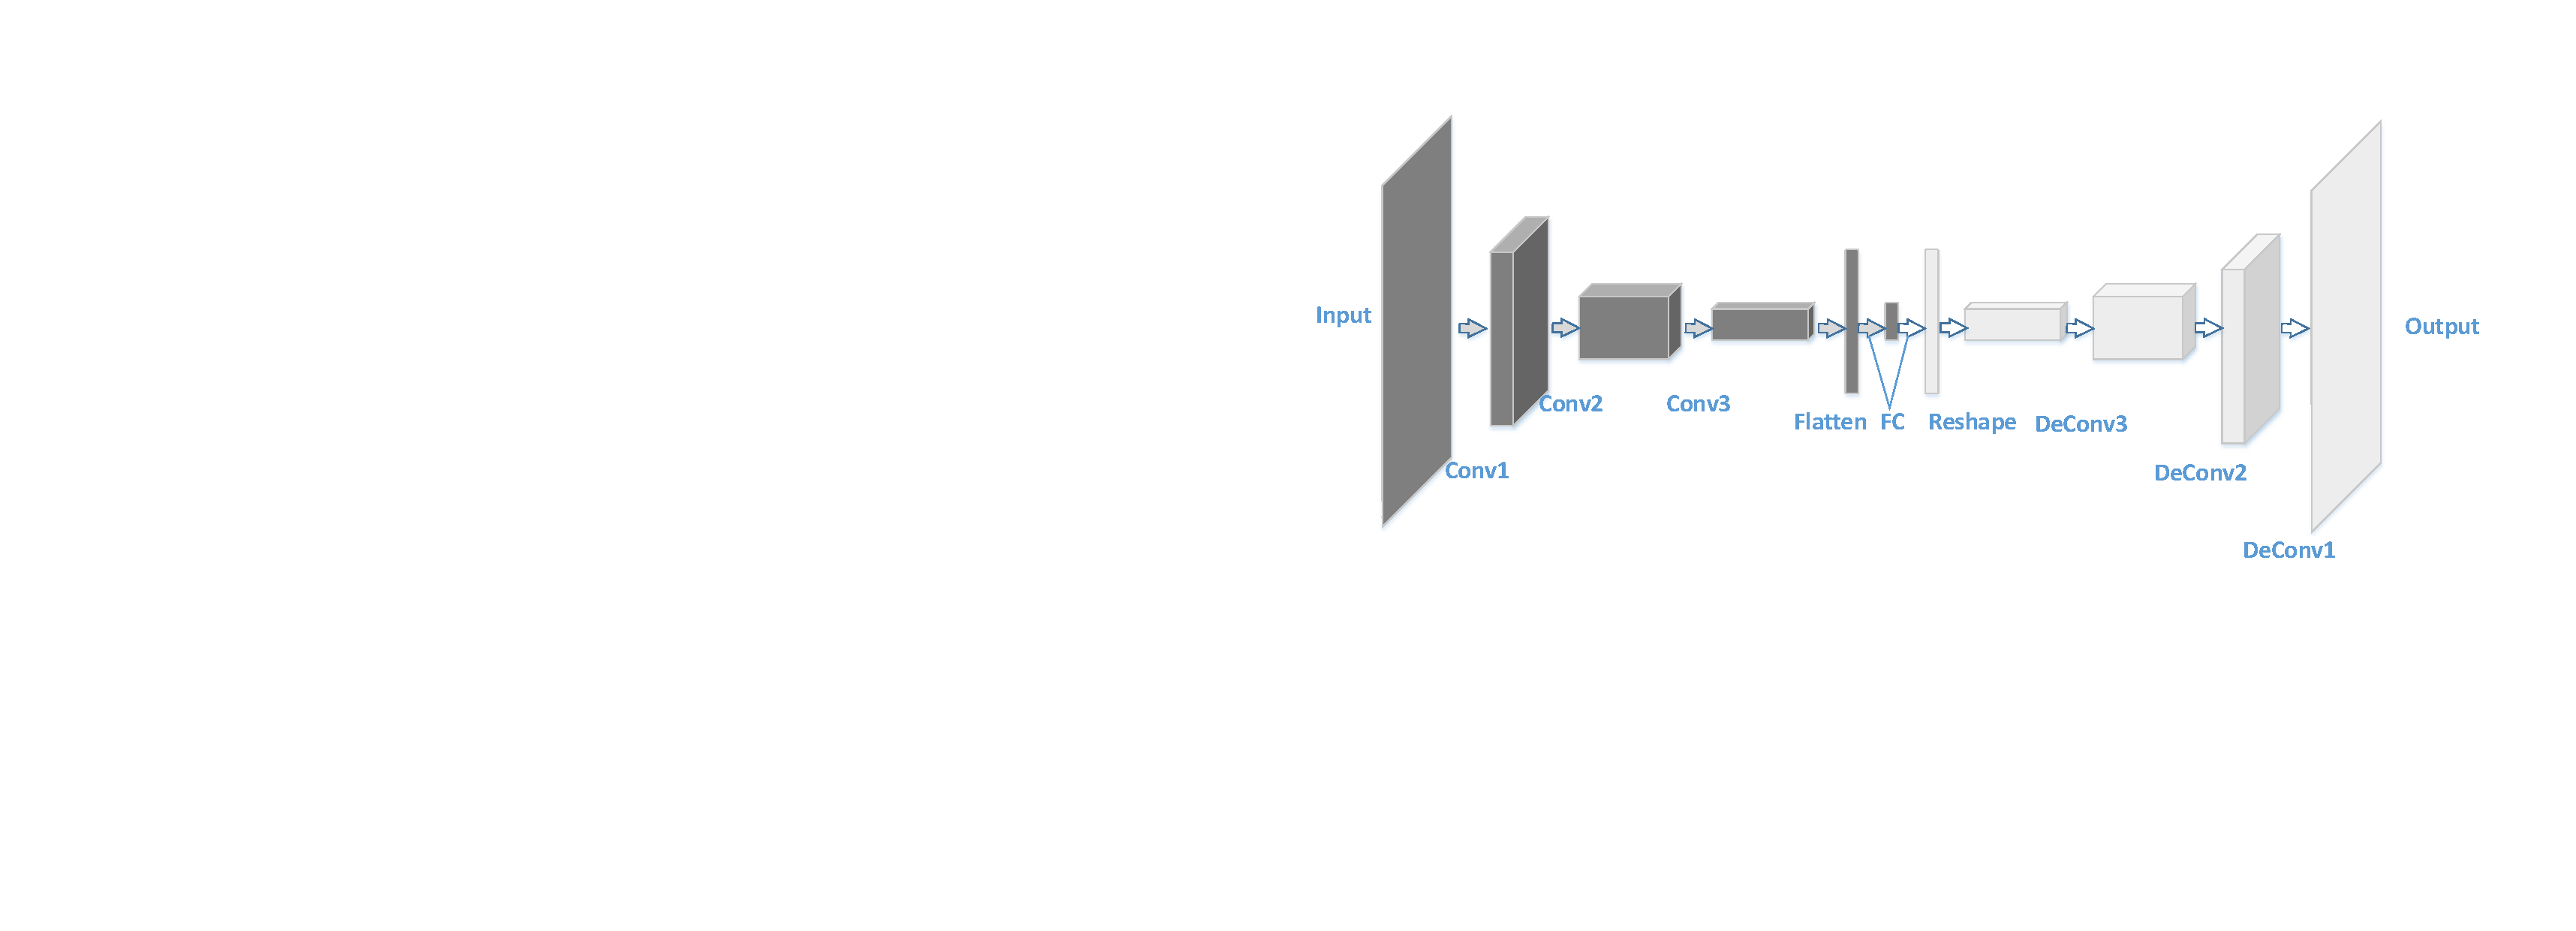
\includegraphics[width=0.92\textwidth]{figures/CAE.pdf}
	\caption{卷积自编码网络示意图}
	\label{fig:CAE}
\end{figure}

逆卷积操作原理如图\ref{fig:conv_dconv}所示,逆卷积操作可以看出是常规卷积操作的逆过程,不同点在于,为了还原原始输入的尺寸,通常需要进行填充(padding)操作(如图\ref{fig:dconv}中的空白区域)。


\begin{figure}[htb]
	\centering
	\subfloat[卷积操作]{\label{fig:conv}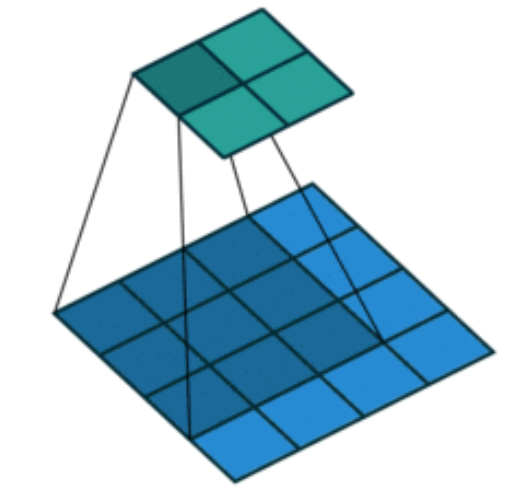
\includegraphics[width=0.42\textwidth]{figures/conv.png}} \qquad
	\subfloat[逆卷积操作]{\label{fig:dconv}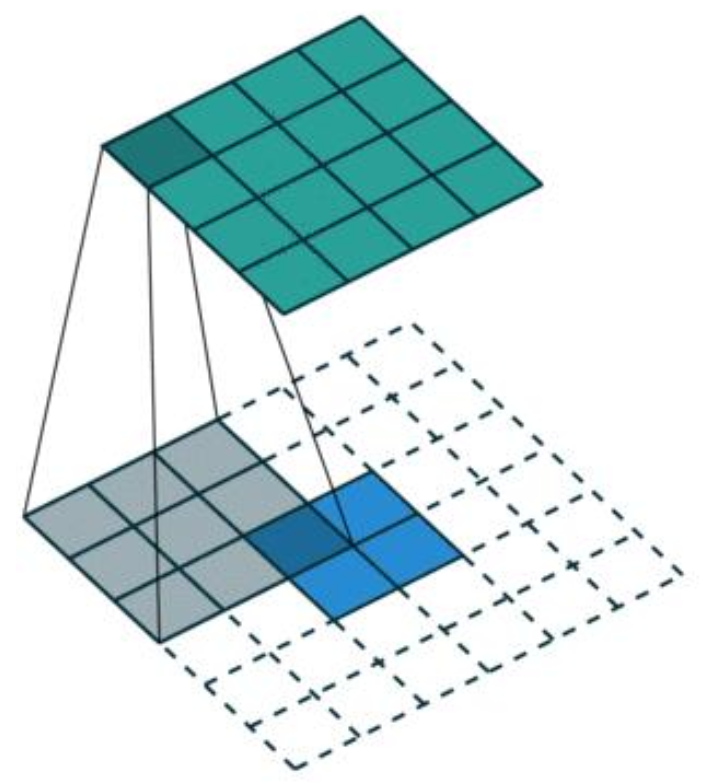
\includegraphics[width=0.38\textwidth]{figures/dconv.png}} 
	\caption{逆卷积操作原理}
	\label{fig:conv_dconv}
\end{figure}

%\begin{figure}[htp]
%	\centering
%	%\includegraphics[width=0.42\textwidth]{data/MLP.pdf}
%	subfigure[卷积操作]{\label{fig:conv}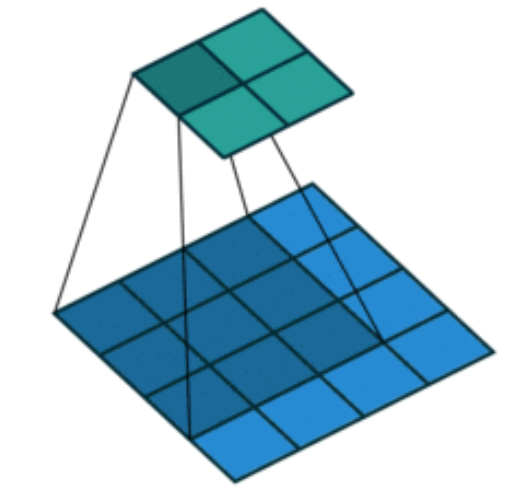
\includegraphics[width=0.42\textwidth]{figures/conv.png}}
%	subfigure[逆卷积操作]{\label{fig:dconv}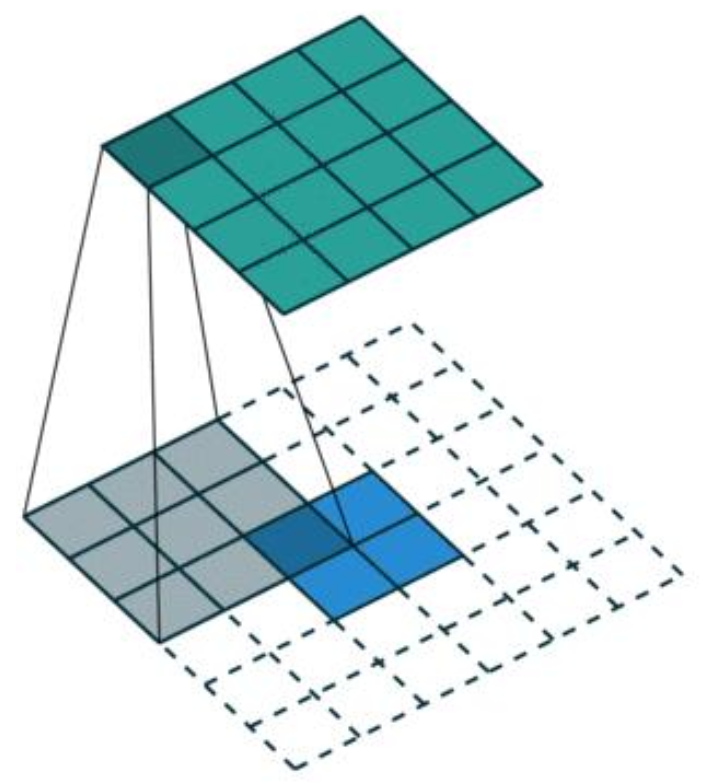
\includegraphics[width=0.42\textwidth]{figures/dconv.png}}
%	\caption{逆卷积操作原理}
%	\label{fig:conv_dconv}
%\end{figure}


对于无监督学习,在卷积神经网络的编码器和解码器的衔接处,利用全连接层,也可以提取带图像数据特征表示;在进行有监督学习时,网络更关注解码器的输出$Y^{\prime}$而不是z,损失函数转化为:
\begin{equation}
Loss_{MSE} = \min _{\phi, \theta}\left\|Y-Y^{\prime}\right\|_{2}^{2}
\end{equation}
从而可以利用卷积神经网络进行有监督学习任务,在气动流场模拟领域已有基于卷积自编码网络开展的工作\cite{DBLP:conf/kdd/GuoLI16}。



\subsection{基于深度学习的图像分割模型}
图像分割一直是计算机视觉领域的难题,也是该领域的研究热点。
所谓图像分割是指根据灰度、彩色、空间纹理、几何形状等特征把图像划分成若干个互不相交的区域,使得这些特征在同一区域内表现出一致性或相似性,而在不同区域间表现出明显的不同。
传统的方法有基于阈值的分割方法;基于区域的图像分割方法;基于边缘检测的分割方法;基于小波分析和小波变换的分割方法;基于遗传算法的分割方法等\cite{图像分割方法综述}。

近年来,深度学习方法开始应用到图像分割,通过搭建神经网络,对训练样本进行有监督学习,得到图形分割的模型。根据分割应用任务不同,图像分割分可分为普通分割、语义分割和实例分割。其中:普通分割是指对分属不同区域的像素点进行分类;语义分割是在分类的基础上识别出每一块区域的语义;实例分割在在语义分割的基础上,进一步对每个识别目标进行编号。本节重点介两种经典的语义分割网络:全卷积网络和U-net网络,分别适用于自然图像分割和医疗图像分割。


\subsubsection{全卷积网络}
2015年Long等人提出的全卷积网络(Fully Convolutional Networks,FCN)用于图像语义分割\cite{Long2015Fully}。自从提出后,FCN已经成为语义分割的基本框架,后续算法都借鉴了该框架的思想。

\begin{figure}[htp]
	\centering
	%\includegraphics[width=0.42\textwidth]{data/MLP.pdf}
	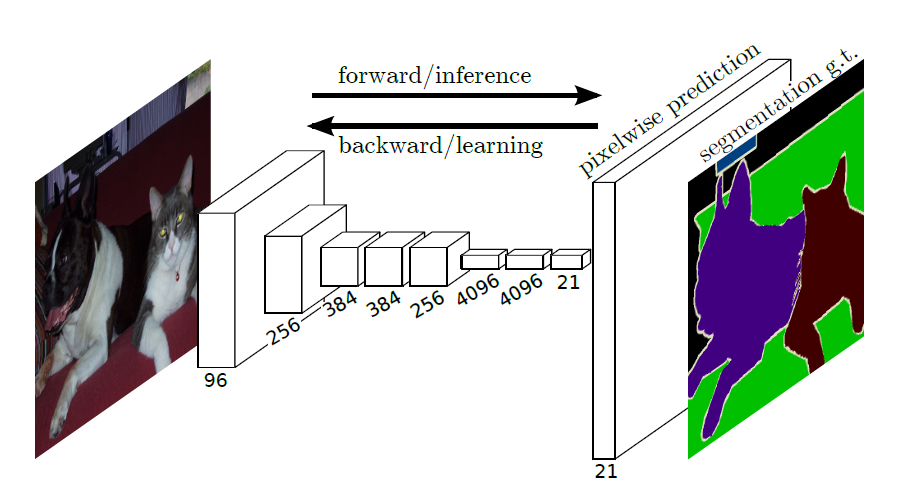
\includegraphics[width=0.88\textwidth]{figures/FCN.png}
	\caption{FCN网络结构图}
	\label{fig:FCN}
\end{figure}

如图\ref{fig:FCN}所示,FCN参考了图像分类网络中的VGG16\cite{2014Very}网络架构。图像分类网络只能对整个图片进行分类而不能识别每个像素点的类别。
为了实现逐像素分类的目的,FCN用卷积层替换了VGG网络中的全连接层,最后利用逆卷积的上采样方法将特征图恢复成原始图片大小,从对整张图片的稀疏分类转换成对每个像素点进行密集分类(dense prediction),达到图像分割的目的。

FCN的另一个特点是利用了全局信息和局部信息。经过多次卷积和池化操作以后,得到的图像越来越小,分辨率越来越低,最后产生了高维特征图。如果直接对进行上采样至原始图片大小,会产生模糊的分割结果。为了解决这一问题,FCN使用了如图\ref{fig:FCN_skip}所示的skip layer的方法。

对于FCN-32s,高层得到的粗糙层(conv7)进行32倍上采样操作,再对每个点进行softmax逻辑回归处理,得到每一个像素点的分类。

对于FCN-16s,先将conv7的结果进行2倍上采样,再将上采样结果与浅层的精细层(pool4)进行逐点相加,最后进行16倍的上采样操作得到与原始输入尺寸相同的图像分割结果。

对于FCN-8s,先将conv7的结果进行4倍上采样,将pool4的结果进行2倍上采样,再将上采样结果与更浅层的精细层(pool3)进行逐点相加,最后进行8倍上采样操作和softmax处理。

通过skip layer的方法,融合多层特征图,有效整合了粗粒度的语义信息和细粒度的位置信息,有利于提高分割准确性。
尽管8倍上采样的FCN的分割效果已经有了很大提升,但是结果还是比较模糊,对分割区域边界不敏感;此外,对每个像素点单独进行分类,没有充分考虑图像的空间上的联系。

\begin{figure}[htp]
	\centering
	%\includegraphics[width=0.42\textwidth]{data/MLP.pdf}
	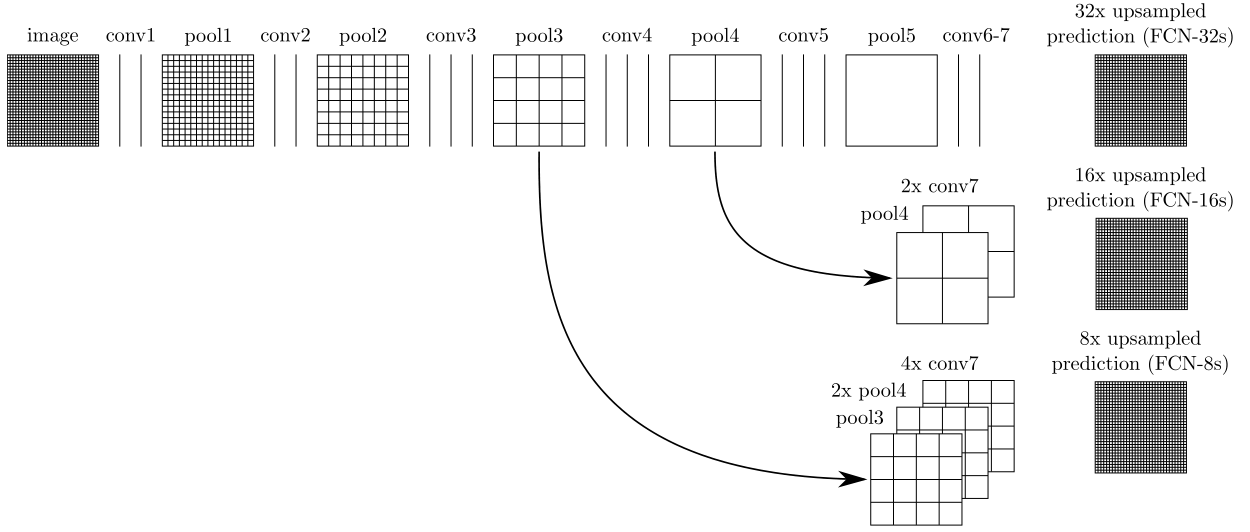
\includegraphics[width=0.88\textwidth]{figures/FCN_skip.png}
	\caption{FCN采用的skip layer方法}
	\label{fig:FCN_skip}
\end{figure}

\subsubsection{U-net网络}
2015年,Ronneberger等人\cite{DBLP:conf/miccai/RonnebergerFB15}提出了U-net网络结构,U-net是基于FCN的一种语义分割网络,适用于做医学图像的分割。U-net修改并扩展了FCN网络结构,使它在使用少量的数据进行训练的情况下获得精确的分割结果。
其主要思想是在下采样网络的后面补充一个对称的上采样网络,多个上采样层增加了网络的参数和表示能力,有利于提升输出结果的分辨率。
对称的网络结构形似英文字母“U”,所以被称为U-net。

U-net网络结构如图\ref{fig:unet}所示:
蓝/白色框表示特征图;蓝色箭头表示3x3卷积层,用于特征提取;灰色箭头表示 skip-connection,用于特征融合;红色箭头表示池化层,用于降低维度;绿色箭头表示上采样 upsample,用于恢复维度;青色箭头表示1x1卷积,用于输出结果。其中灰色箭头中的copy就是atenate操作,将深层的特征图和浅层的特征图在通道方向拼接;crop是为了让两者的长宽一致,保证拼接后的特征图大小一致。


\begin{figure}[htp]
	\centering
	%\includegraphics[width=0.42\textwidth]{data/MLP.pdf}
	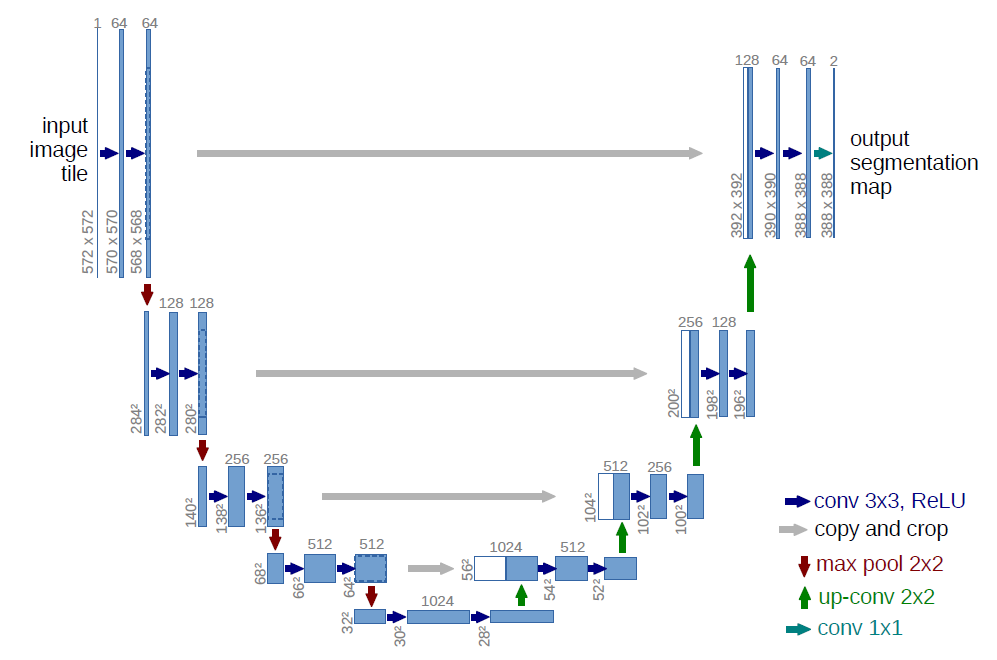
\includegraphics[width=0.88\textwidth]{figures/unet.png}
	\caption{U-net网络结构图\cite{DBLP:conf/miccai/RonnebergerFB15}}
	\label{fig:unet}
\end{figure}

U-net主体结构包括一个捕获上下文信息的收缩路径和一个允许精确定位的对称拓展路径:
收缩部分和扩展部分都有4个采样层。这种架构延续了Encoder-Decoder的思想。
Encoder由卷积操作和下采样操作组成,文中所用的卷积结构统一为3x3的卷积核,填充为 0,步长为1;Decoder部分采用的上采样的方式与FCN中的反卷积不同,为双线性插值。
此外,为了更好融合位置信息和语义信息,U-net拓展了FCN中skip layer的思想,在“U”形网络的对称部分添加了skip connection。与FCN的加操作不同,U-net使用了叠操作(concatenation)增加了特征的厚度,保留了更多浅层的位置信息,这使得上采样层可以在浅层特征与深层特征在训练时进行自适应选择,这对语义分割任务来说更有优势。

由于在医疗图像分割上取得巨大成功,许多研究者针对不同的图像分割任务对U-net进行了改进,产生了许多U-net变体包括V-Net\cite{2016V}、UNet++\cite{unet++}、U-NetPlus\cite{unetplus}和3D U2-Net\cite{20193D}等,提升了模型的推理速度和精度。


\subsection{Pix2Pix网络模型}
对于气动流场预测,核心问题是实现从输入到输出的映射。
除了前文提到的自编码网络和图像分割网络,基于生成对抗网络(Generative Adversarial Network, GAN)的图像风格迁移模型也在解决像素到像素的映射问题上展示出的强大潜力。
GAN在图像生成、风格迁移、超分辨重建等领域已经得到了广泛的应用,
本节我们重点介绍Pix2Pix网络模型\cite{isola2017image}。

Pix2Pix网络基于条件生成对抗网络(Conditional Generative Adversarial Network, cGAN)\cite{cGAN},通过添加条件约束信息来指导完成图像转换任务,比如从标签图合成相片,从线稿图重构对象,给图片上色等。
和传统的GAN网络类似,在Pix2Pix模型训练过程中,迭代地训练生成器和判别器,生成器尽可能生成接近真实的样本,企图“欺骗”判别器;判别器尽可能识别出真实的样本和生成的样本,获得更高的得分。这样的对抗训练过程类似博弈游戏,随着训练的进行,生成器和判别器的能力不断提升直到达到令人满意的效果。
由于添加了约束条件,Pix2Pix网络的输入不再是普通GAN网络中的随机变量,其网络结构示意图
如图\ref{fig:cgan}所示:

\begin{figure}[htp]
	\centering
	%\includegraphics[width=0.42\textwidth]{data/MLP.pdf}
	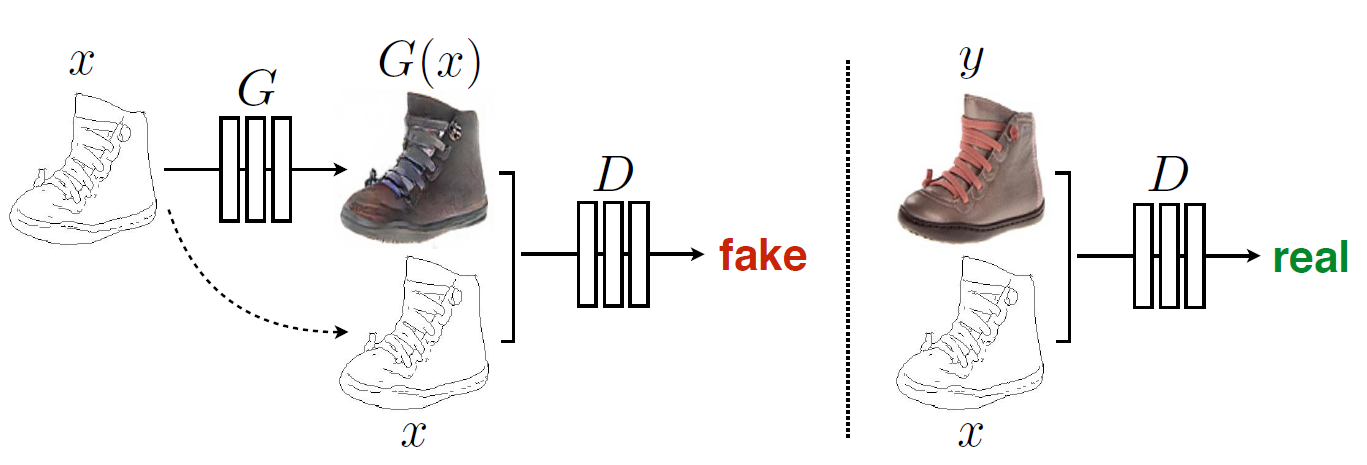
\includegraphics[width=0.88\textwidth]{figures/cGAN.png}
	\caption{Pix2Pix网络结构示意图}
	\label{fig:cgan}
\end{figure}

其中x是条件输入,y是对应的标签,每个输入x唯一对应一个标签y。
在训练生成器时,x进过生成器$G$得到生成图像$G(x)$;
在训练判别器时,输入x和对应生成图像$G(x)$或标签y通过通道维度的叠操作进行拼接,一同送入判别器,判别器会输出概率值,表示是否为一对真实样本。



Pix2Pix网络利用类似U-net的结构代替自编码网络作为生成器,
在输入和输出之间存在很多可以共享的低级信息,采用skip-connection的结构有利于传递这些底层信息和重构图像。
对于判别器网络,Pix2Pix提出了PatchGAN架构。
传统GAN判别器通常对生成样本整体进行判断,对于图片而言,直接输出整张图片是真实样本的概率。而图像转换任务中关注像素到像素的转换效果,所以在这里提出了分块判断的算法,在图像的每个块上去判断是否为真,输出平均预测结果。


条件GAN采用的损失函数通常为:
\begin{equation}
\begin{aligned}
\mathcal{L}_{c G A N}(G, D)= &\mathbb{E}_{x,y}[\log D(x,y)]+\\
&\mathbb{E}_{x,z }[\log (1-D(x, G(x,z))]
\end{aligned}
\end{equation}

\begin{equation}
\begin{aligned}
\mathcal{L}_{c G A N}(G)= \mathbb{E}_{x,z}[\log (1-D(x, G(x, z))]
\end{aligned}
\end{equation}

\noindent 其中z为输入随机变量,在Pix2Pix网络输入仅为x。
此外,为了保证像素级低频信息的预测精度,Pix2Pix网络的损失函数还引入了$L_1$损失项:

\begin{equation}
\begin{aligned}
\mathcal{L}_{L 1}(G)=\mathbb{E}_{x_1, x_2, y}\left[\|y-G(x_1, x_2)\|_{1}\right]
\end{aligned}
\end{equation}

考虑到训练的最终目标是获得一个性能良好的生成器,同时生成器和判别器进行着对抗的训练,所以训练的最终目标是:
\begin{equation}
\begin{aligned}
G^{*}=\arg \min _{G} \max _{D} \mathcal{L}_{c G A N}(G, D)+\lambda \mathcal{L}_{L 1}(G)
\end{aligned}
\end{equation}
\noindent 其中$\lambda$是$L_1$损失函数项的权重系数。


\subsection{图卷积神经网络}

在深度学习发展过程中,卷积神经网络(Convolutional Neural Network, CNN)和循环神经网络(Recurrent Neural Network, RNN)在图像识别、语义分割、自然语言处理等领域发挥了重要作用。
无论是图像还是语言,在CNN或RNN进行处理时都被转换成结构规则的数据形式,都属于欧式空间的数据。
然而现实生活中有很多不规则的数据结构,如社交网络、化学分子结构、生物网络等;即使是语言,其内部实际是复杂的树形结构,
只是RNN将其处理成向量的形式便于神经网络训练。
图结构通常被用来表示这些非欧式空间的数据,但是在图结构中,每个节点周围的结构千差万别,不同于图像和向量化的语言数据具有平移不变性,因此不可能直接利用CNN或RNN进行处理。

近年来,人们对深度学习方法在图上的拓展进行了大量的研究,研究人员借鉴CNN、RNN以及图嵌入技术的思想,
定义和设计了专用于处理图结构数据的神经网络,即图神经网络(Graph  Neural  Network, GNN)。
文献\cite{2019A}将GNN分为五大类:图卷积网络(Graph Convolution Networks,GCN)、 图注意力网络(Graph Attention Networks)、图自编码器( Graph Autoencoders)、图生成网络( Graph Generative Networks) 和图时空网络(Graph Spatial-temporal Networks)。
本节重点介绍图卷积神经网络。

GCN方法主要分为两大类,基于谱(spectral-based)和基于空间(spatial-based)。
基于谱的方法将空域信号利用傅里叶变换转换到频域进行分析处理,完成在空域无法完成的操作。
对于无向图有正则化拉普拉斯矩阵:

\begin{equation}
\mathbf{L}=\mathbf{I}_{\mathbf{n}}-\mathbf{D}^{-\frac{1}{2}} \mathbf{A} \mathbf{D}^{-\frac{1}{2}}
\end{equation}

\noindent $I_n$为单位矩阵,A为图的邻接矩阵,D为对角矩阵。
对L进行特征值分解有:

\begin{equation}
\mathbf{L}=\mathbf{U} \mathbf{\Lambda} \mathbf{U}^{T}
\end{equation}

\noindent U是特征向量构成的矩阵,$\Lambda$是对角矩阵,对角线上的值为L的特征值。
对输入图信号x的傅里叶变换和傅里叶逆变换分别被定义为

\begin{equation}
\mathfrak{F}(\mathrm{x})=\mathbf{U}^{T} \mathrm{x} 
\end{equation}
\begin{equation}
\mathfrak{F}^{-1}(\hat{\mathrm{x}})=\mathbf{U} \hat{\mathrm{x}}
\end{equation}

\noindent $\hat{\mathrm{x}}$为傅里叶变换的结果。
定义对输入图信号的图卷积操作为:

\begin{equation}
\begin{aligned}
\mathrm{x} *_{G} \mathrm{g} &=\mathfrak{F}^{-1}(\mathfrak{F}(\mathrm{x}) \odot \mathfrak{F}(\mathrm{g})) \\
&=\mathbf{U}\left(\mathbf{U}^{T} \mathrm{x} \odot \mathbf{U}^{T} \mathrm{g}\right)
\end{aligned}
\end{equation}
\noindent 其中g是定义的滤波器,$\odot$表示哈达玛积运算。
基于频谱的图卷积网络都遵循这样的模式,它们之间关键的不同点在于选择的滤波器不同
基于谱的方法从图信号处理的角度引入滤波器来定义图卷积,根据图谱理论和卷积定理,将数据由空域转换到谱域做处理,理论基础坚实。
基于空间的方法将图卷积表示为从邻域聚合特征信息,直接在图空间上定义卷积操作,灵活性更强。




\begin{figure}[htp]
	\centering
	%\includegraphics[width=0.42\textwidth]{data/MLP.pdf}
	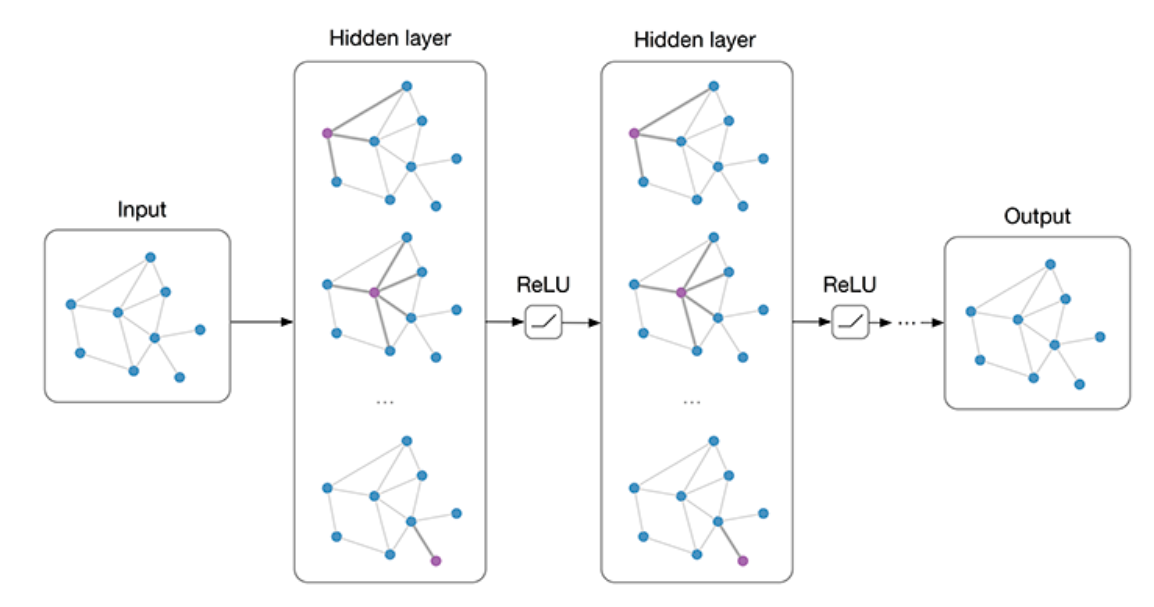
\includegraphics[width=0.88\textwidth]{figures/GCN.png}
	\caption{多层GCN网络示意图}
	\label{fig:gcn}
\end{figure}

对于图卷积算法的实现主要包括三个步骤:
\romannumeral1)发送:每一个节点将自身的特征信息经过变换后发送给邻居节点。这一步是在对节点的特征信息进行抽取变换;
\romannumeral2)接收:每个节点将邻居节点的特征信息聚集起来。这一步是在对节点的局部结构信息进行融合;
\romannumeral3)变换:把前面的信息聚集之后做非线性变换,增加模型的表达能力。
图\ref{fig:gcn}展示了一个简单的GCN网络,从图中可以发现数据的拓扑结构在训练过程中始终保持不变,
可以在训练中重复利用。
每一层的节点特征维度是不固定的,可以根据训练任务的复杂程度进行灵活的调整。

概括而言,图卷积算子的作用就是将每个节点的特征与其邻居节点的特征加权平均后传播到下一层,具有以下特点:
1)局部参数共享,计算节点特征值时,按一定规律将参与聚合的节点分为若干个子集,
同一个子集内的节点采用相同的权重;
2)节点感受域正比于层数,每一层图卷积运算只能和相邻的节点进行特征聚合;通过增加GCN层数,每个节点上参与运算的其他节点信息就更多;
3)适用于任意拓扑结构的节点与图,能同时对节点特征信息与图结构信息进行端对端学习。


%\section{实验算例介绍}
%\subsection{2D不可压层流固体外部流场}
%\subsection{2D不可压有粘翼型外部流场}



\section{本章小结}

本章首先通过对比传统CFD求解器和基于深度学习的气动优化模型的工作流程,明确了利用深度学习技术和方法要解决的CFD问题。
然后介绍了CFD相关理论知识,重点介绍了在宏观和介观层面对流体运动规律的描述。
最后分析了气动流场模拟任务和深度学习中图像回归预测任务的相似性,介绍了与本文研究内容紧密相关的深度网络模型。








%%% Local Variables:
%%% mode: latex
%%% TeX-master: "../main"
%%% End:

\begin{ack}
行文至此,硕士研究生学习生活已经接近尾声。在毕设论文完成之际,谨向这两年半时间里在生活学习等各方面给予我支持与帮助的人表示最衷心的感谢!

首先,感谢两年半前的自己,是你之前的努力换来了打开国防科大研究生生活大门的钥匙,让我有幸在一个高规格、高水平和高层次的平台继续深造。

感谢我的硕士指导老师邓小刚老师!邓老师学识渊博,治学严谨。
在毕设选题和研究内容上进行了建设性的指导,在课题研究方向和研究方法提出了宝贵的建议。
邓老师对待学术研究态度严谨、一丝不苟的品格也一直激励着我不断在研究领域进行探索,跟随邓老师进行学术研究的两年半获益匪浅。

由衷感谢课题组的徐传福老师!从硕士入学到即将毕业徐老师一直悉心指导和周密安排,无论生活中还是实验上遇到难处,徐老师都会积极开导,帮助解决,每次与之交流都收获颇丰。
在组会讨论时,徐老师都会认真倾听汇报并给出针对性建议,及时帮助我解决课题研究中遇到的困难。徐老师是我硕士生涯的引路人,一步一步指引我在学术研究上不断取得突破。

感谢方建滨师兄和高翔师兄!两位师兄分别在我硕士前后阶段对我的研究工作进行了细致耐心的指导,传授了许多宝贵的学习经验,让我少走了不少弯路。两位优秀的师兄有着严谨的治学态度和良好的生活学习习惯,一直是我学习看齐的榜样!

感谢课题组陈世钊师兄,帮助解决了生活和学习中很多难题,从钊哥身上学习到很多为人处世的方法!感谢课题组熊敏、程彬、郭宁波、林玉、刘舒、苗秋成、张海红、顾善植等师兄师姐,在学习和生活上提供很多指导!感谢课题组廖海翔、郭睿、史玮三位同级,在日常工作和学习上大家相互配合相互促进!感谢课题组王啸宇、高婉蓉、李文强、朱东等师弟师妹,有了你们实验室的学习生活不再单调枯燥。

感谢203小分队成员郭凌超、黄永钦和李晨,两年半以来我们同甘共苦,从你们身上我学到很多,是你们解决我生活的后顾之忧,为生活增添了很多乐趣。

感谢我的父母,一直无条件支持我、鼓励我、爱我,为我提供了温馨幸福的生活条件,解决了我学习和工作的后顾之忧。

最后感谢我的女朋友张燕平,谢谢你的一直陪伴和支持,牺牲和理解,包容和爱。


\end{ack}


\cleardoublepage
\phantomsection
\addcontentsline{toc}{chapter}{参考文献}
\ifisbiber
{\hyphenpenalty=500 %
\tolerance=9900 %
\renewcommand{\baselinestretch}{1.35}
\printbibliography[heading=bibliography, title=参考文献]

}
\else
\bibliographystyle{bstutf8}
\bibliography{ref/refs}
\fi

\begin{resume}
\ifreview
该论文作者在学期间取得的阶段性成果(学术论文等)已满足我校硕士学位评阅相关要求。为避免阶段性成果信息对专家评价学位论文本身造成干扰,特将论文作者的阶段性成果信息隐去。
\else

\ifisresumebib

	\begin{refsection}[ref/resume.bib]
	\settoggle{bbx:gbtype}{false}%局部设置不输出文献类型和载体标识符
	\settoggle{bbx:gbannote}{true}%局部设置输出注释信息
	\setcounter{gbnamefmtcase}{1}%局部设置作者的格式为familyahead格式   
	\nocite{ref-1-1-Yang,ref-2-1-杨轶,ref-3-1-杨轶,ref-4-1-Yang,ref-5-1-Wu,ref-6-1-贾泽,ref-7-1-伍晓明}
	
	\setlength{\biblabelsep}{12pt}
	\printbibliography[env=resumebib,heading=subbibliography,title={发表的学术论文}] % 发表的和录用的合在一起

	\end{refsection}


	\begin{refsection}[ref/resume.bib]
	\settoggle{bbx:gbtype}{false}%局部设置不输出文献类型和载体标识符
	\settoggle{bbx:gbannote}{true}%局部设置输出注释信息
	\setcounter{gbnamefmtcase}{1}%局部设置作者的格式为familyahead格式
	\nocite{ref-8-1-任天令,ref-9-1-Ren}
	
	\setlength{\biblabelsep}{12pt}
	\printbibliography[env=resumebib,heading=subbibliography,title={研究成果}]

	\end{refsection}

\else

  \section*{发表的学术论文} % 发表的和录用的合在一起

  \begin{enumerate}[label={[\arabic*]}]
  \addtolength{\itemsep}{-.36\baselineskip}%缩小条目之间的间距,下面类似
  \item \textbf{Donglin Chen}, Xiang Gao, Chuanfu Xu, Shizhao Chen, Jianbin Fang, Zhenghua Wang, and Zheng Wang. 
  FlowGAN: A Conditional Generative Adversarial Network for Flow Prediction in Various Conditions. 
  International Conference on Tools with Artificial Intelligence (ICTAI, CCF C) 2020.

  \item \textbf{Donglin Chen}, Jianbin Fang, Chuanfu Xu, Shizhao Chen, Zheng Wang. 
  Characterizing Scalability of Sparse Matrix-Vector Multiplications on Phytium FT-2000+. 
  International Journal of Parallel Programming (IJPP, SCI IF 1.244, 中科院SCI分区3区). 48(1): 80-97, 2020.
  
  \item \textbf{Donglin Chen}, Jianbin Fang, Chuanfu Xu, Shizhao Chen, Zheng Wang. 
  Optimizing Sparse Matrix-Vector Multiplications on an ARMv8-based Many-Core Architecture. 
  International Journal of Parallel Programming (IJPP, SCI IF 1.244, 中科院SCI分区3区). 47(3): 418-432, 2019.
   
  \item \textbf{Donglin Chen}, Xiang Gao, Chuanfu Xu, Siqi Wang, Shizhao Chen, Jianbin Fang, and Zheng Wang. 
  FlowDNN: A Physics-Informed Deep Neural Network for Fast and Accurate Flow Prediction. 
  (Frontiers of Information Technology \& Electronic Engineering FITEE, SCI under review.)
  
  \item Shizhao Chen, Jianbin Fang, \textbf{Donglin Chen}, Chuanfu Xu, Zheng Wang. 
  Adaptive Optimization of Sparse Matrix-Vector Multiplication on Emerging Many-Core Architectures. 
  IEEE International Conference on High Performance Computing and Communications (HPCC) 2018: 649-658.
  


  \end{enumerate}

%  \section*{研究成果} % 有就写,没有就删除
%  \begin{enumerate}[label=\textbf{[\arabic*]}]
%  \addtolength{\itemsep}{-.36\baselineskip}%
%  \item 任天令, 杨轶, 朱一平, 等. 硅基铁电微声学传感器畴极化区域控制和电极连接的
%    方法: 中国, CN1602118A. (中国专利公开号.)
%  \item Ren T L, Yang Y, Zhu Y P, et al. Piezoelectric micro acoustic sensor
%    based on ferroelectric materials: USA, No.11/215, 102. (美国发明专利申请号.)
%  \end{enumerate}
\fi
\fi
\end{resume}

% 最后,需要的话还要生成附录,全文随之结束。
\appendix
\backmatter
\input{data/appendix01}

\end{document}
